\documentclass[a4paper,UKenglish]{tufte-handout}

\usepackage[utf8]{inputenc}
\usepackage{microtype}
\DisableLigatures{encoding=*,family=tt*}
\usepackage{mathtools}
\usepackage{amsmath}
\usepackage{mathpartir}
\usepackage{agda}
\usepackage{geometry}
\usepackage{hyperref}
\hypersetup{colorlinks=true, linkcolor=black, citecolor=black, filecolor=black, urlcolor=black}
\usepackage[parfill]{parskip}
\usepackage{color,colortbl,xcolor}
\usepackage{booktabs}
\usepackage{amsthm}

\usepackage{tikz}
\usetikzlibrary{positioning}

\newcommand{\hrefu}[2]{\href{#1}{\nolinkurl{#2}}}

\theoremstyle{definition}
\newtheorem{exercise}{Exercise}[section]

\clubpenalty=10000
\widowpenalty=10000
\displaywidowpenalty=10000

\hfuzz=1000pt

\setcounter{secnumdepth}{1}

\usepackage{newunicodechar}
\newunicodechar{→}{\ensuremath{\rightarrow}}
\newunicodechar{←}{\ensuremath{\leftarrow}}
\newunicodechar{×}{\ensuremath{\times}}
\newunicodechar{λ}{\ensuremath{\lambda}}
\newunicodechar{∀}{\ensuremath{\forall}}
\newunicodechar{Π}{\ensuremath{\Pi}}
\newunicodechar{Σ}{\ensuremath{\Sigma}}
\newunicodechar{≡}{\ensuremath{\equiv}}
\newunicodechar{≅}{\ensuremath{\cong}}
\newunicodechar{≐}{\ensuremath{\doteq}}
\newunicodechar{∈}{\ensuremath{\in}}
\newunicodechar{∧}{\ensuremath{\land}}
\newunicodechar{∨}{\ensuremath{\lor}}
\newunicodechar{⊤}{\ensuremath{\top}}
\newunicodechar{⊥}{\ensuremath{\bot}}
\newunicodechar{⊔}{\ensuremath{\sqcup}}
\newunicodechar{∷}{\ensuremath{{::}}}
\newunicodechar{ℓ}{\ensuremath{\ell}}
\newunicodechar{₀}{\ensuremath{{_0}}}
\newunicodechar{₁}{\ensuremath{{_1}}}
\newunicodechar{₂}{\ensuremath{{_2}}}
\newunicodechar{₃}{\ensuremath{{_3}}}
\newunicodechar{₄}{\ensuremath{{_4}}}
\newunicodechar{₅}{\ensuremath{{_5}}}
\newunicodechar{₆}{\ensuremath{{_6}}}
\newunicodechar{₇}{\ensuremath{{_7}}}
\newunicodechar{₈}{\ensuremath{{_8}}}
\newunicodechar{₉}{\ensuremath{{_9}}}
\newunicodechar{⟨}{\ensuremath{{\langle}}}
\newunicodechar{⟩}{\ensuremath{{\rangle}}}
\newunicodechar{̧}{\c}
\newunicodechar{∘}{\ensuremath{\circ}}

\newcommand\var[1]{\mathit{#1}}
\newcommand\prim[1]{{\AgdaPrimitive{#1}}}
\newcommand\ty[1]{{{\prim{Set}}_{#1}}}
\newcommand\fun[1]{{\AgdaFunction{#1}}}
\newcommand\data[1]{{\AgdaFunction{#1}}}
\newcommand\con[1]{{\AgdaInductiveConstructor{#1}}}
\newcommand\field[1]{{\AgdaField{#1}}}
\newcommand\keyw[1]{{\AgdaKeyword{#1}}}
\newcommand\lit[1]{{\AgdaNumber{#1}}}
\newcommand\level{\fun{Level}}
\newcommand\ite[3]{\fun{if}\  #1\  \fun{then}\  #2\  \fun{else}\  #3}

\newcommand\Nat{\data{Nat}}
\newcommand\zero{\con{zero}}
\newcommand\suc{\con{suc}}
\newcommand\Bool{\data{Bool}}
\newcommand\true{\con{true}}
\newcommand\false{\con{false}}
\newcommand\List{\data{List}}
\renewcommand\Vec{\data{Vec}}
\newcommand\nil{\con{[]}}
\newcommand\cons{\con{::}}
\newcommand\Fin{\data{Fin}}
\renewcommand\prod{\data{×}}
\newcommand\sigmatype{\data{Σ}}
\newcommand\toptype{\data{⊤}}
\newcommand\bottomtype{\data{⊥}}
\newcommand\Id{\data{≡}}
\newcommand\refl{\con{refl}}


\title{Programming and Proving in Agda}
\author{Jesper Cockx}
\date{Version of \today}

\begin{document}


\begin{code}[hide]
{-# OPTIONS --allow-unsolved-metas #-}
\end{code}

\maketitle

\begin{abstract}
Agda is both a strongly typed functional programming language with
support for first-class \emph{dependent types} and a \emph{proof
assistant} based on the Curry-Howard correspondence between
propositions and types. The goal of these lecture notes is to introduce both
these unique aspects of Agda to a general audience of functional
programmers. It starts from basic knowledge of Haskell as taught in
Hutton's book \emph{Programming in Haskell}, and builds up to
using equational reasoning to formally prove correctness of
functional programs.
\end{abstract}

\tableofcontents
\clearpage

\section{An introduction to Agda for Haskell programmers}

Most programmers think of a type system as a set of rules that
together prevent a class of basic runtime errors, such as using a
string where the program expects an integer. This is indeed why type
systems were first introduced to programming languages: to prevent
program crashes that would follow from interpreting data in memory
incorrectly.\footnote{For example, a type system can prevent the
floating point number $1.0$ from being interpreted as a memory
address.}  However, since their invention, type systems have evolved
to include a much broader range of applications:

\begin{itemize}

\item By making use of type information, an IDE can help the
programmer during the programming by providing type information and
suggestions and by generating and modifying code based on the type
information. For example, the IDE can use types to generate all
possible cases in a case expression.

\item A type can express precise invariants of data in a program, such
as the length of a list or the lower and upper bounds of a search
tree. These expressive types that can depend on runtime inputs are
known as \emph{dependent types}.

\item Types can even be used to express mathematical properties and
proofs of these properties, which can be checked automatically by the
type checker. This usage of a type system as a logic is based on a
deep and fundamental result known as the \emph{Curry-Howard
correspondence}.

\end{itemize}

While strongly typed languages such as Java or Haskell have type
systems that are quite expressive, due to various reasons it is hard
to fully appreciate the three above points from their
perspective. In these lecture notes, we will study Agda, a functional language that
is similar to Haskell but is a bit more experimental and has an even
more expressive type system with full support for dependent types.

On the surface level, Agda code looks quite similar to Haskell code,
with some small syntactic differences. However, beneath the hood are a
number of notable differences:
\marginnote{%
\paragraph{Historical note.} Agda's type system is based on
\emph{dependent type theory}, a formal language invented by the
Swedish philosopher Per Martin-L\"of. His original motivation was to
provide a new foundation for \emph{constructive mathematics}, a kind
of mathematics where each proof of existence contains an algorithm to
actually construct the object that is proven to exist. For example, a
constructive proof of ``there exists a prime number greater than
1000'' provides an algorithm to actually produce such a number. Later
on, it was discovered that Martin-L\"of's type theory is also well
suited to implement computer proof assistants (such as the Coq system)
and programming languages with built-in support for verification (such
as Agda).
}
\begin{itemize}

\item Types in Agda are \emph{first-class values}: basic types such as
  $\Nat$ and $\Bool$ are themselves values of another type called
  $\ty{}$. Values of type $\ty{}$ can be passed around as arguments
  and returned just as other values.

\item All functions in Agda are \emph{total}: where evaluating a
  function call in Haskell could lead to a runtime error or loop
  forever, evaluating a function call in Agda is guaranteed to always
  return a value of the correct type in finite time.

\item Agda has support for \emph{dependent function types} where the
  type of the output can be different depending on the runtime value
  of the input. This allows us to assign a precise type to functions
  that are impossible to type correctly in many other languages, such
  as $\fun{printf}$.

\item Agda also has types that correspond to (proofs of) \emph{logical
  propositions}. Using these types, Agda can also be used as a
  \emph{proof assistant} for writing and checking mathematical proofs.

\end{itemize}


The goal of these lecture notes is \emph{not} to provide a full guide to using
Agda as a full-featured programming language. Instead, we use Agda as a vehicle
to study the basic building blocks that make up a dependently typed functional
programming language. Most of the types and functions we define --- as well as
much more --- can be found in Agda's standard library, which you can get from
\hrefu{https://github.com/agda/agda-stdlib}{github.com/agda/agda-stdlib}. In
these notes, we will not make use of the standard library and instead define
everything from the ground up. When using Agda for real, it is of course
much easier to get these definitions from the library instead!


\subsection{Installing Agda}

There are several ways to install Agda, but unfortunately none are
very fast and simple. Here we describe how to install Agda from source
using Stack.\footnote{Instructions for installing Stack can be found
on \hrefu{https://docs.haskellstack.org/en/stable/README/}{docs.haskellstack.org/en/stable/README}.} Other ways
to install Agda can be found at
\hrefu{https://agda.readthedocs.io/en/latest/getting-started/installation.html}{agda.readthedocs.io/en/latest/getting-started/installation.html}.
To follow the rest of these notes, it is recommended that you use
Agda version 2.6.0 or later.

Assuming you have Stack installed, the following command should install the
latest release of Agda:
\begin{verbatim}
stack install Agda-2.6.1.3
\end{verbatim}
This step will take a long time and a lot of memory to complete, and
use up 4-5 GB of disk space for a fresh install.

On Ubuntu Linux and similar systems (including
WSL\footnote{\hrefu{https://docs.microsoft.com/en-us/windows/wsl/install-win10}{docs.microsoft.com/en-us/windows/wsl/install-win10}}
on Windows) you can alternatively install a binary release by running
`\texttt{sudo apt install agda}`.

To write and edit Agda code, we recommend Visual Studio Code with the
\texttt{agda-mode} extension.\footnote{You can get Visual Studio Code
from \hrefu{https://code.visualstudio.com/}{code.visualstudio.com}. To install an extension,
click the Extensions button on the left, enter the name of the
extension, and click `install'.} Other IDEs with support for Agda are
Emacs and Atom.

You can test to see if you’ve installed Agda correctly by creating a file
called \texttt{hello.agda} with these lines:

\begin{code}[number]
data Greeting : Set where
  hello : Greeting

greet : Greeting
greet = hello
\end{code}
Open this file in VS Code and press the key combination
\texttt{Ctrl+c} followed by \texttt{Ctrl+l} (for ``load file''). You
should see a new frame titled Agda with the message \texttt{*All
Done*}, and the code should be highlighted.\footnote{In this
introduction to Agda we will only use the interactive mode of Agda,
which acts as a type checker and interpreter similar to \texttt{ghci}
for Haskell. Agda also supports several backends for compilation,
including a GHC backend and a JavaScript backend. A full ``Hello,
world'' example for creating an executable from your Agda code can be
found at
\hrefu{https://agda.readthedocs.io/en/v2.6.1.3/getting-started/hello-world.html}{agda.readthedocs.io/en/v2.6.1.3/getting-started/hello-world.html}.}

Once you have loaded an Agda file, there is a number of other commands that
can be used to query the typechecker. Here are two that are used very often:

\begin{description}
\item[Deduce type (\texttt{Ctrl+c Ctrl+d})] This command will ask you
  for an expression, for which it will then try to infer the type. For
  example, running this command and entering \texttt{hello} will
  return the inferred type \texttt{Greeting}.
\item[Normalize expression (\texttt{Ctrl+c Ctrl+n})] This command will ask you
  for an expression, which it will evaluate as far as possible. For
  example, running this command and entering \texttt{greet} will
  return the fully evaluated term \texttt{hello}.
\end{description}

Since there is no syntactic difference between values, functions, and types in
Agda, it can be difficult at first to determine what kind of expression you are
dealing with. If you run into such a situation, try first to predict its type
and normal form, and then use the commands above to test your prediction.

\subsection{Syntactic differences with Haskell}

As we noted before, the syntax of Agda is in many respects similar to
that of Haskell. Here we list the most important differences:

\begin{description}

\item[Typing] Typing is denoted by a single colon in Agda. For example, instead
of writing \texttt{b ::~Bool} as in Haskell, in Agda we write $\fun{b} : \Bool$
to indicate that \fun{b} is a boolean.

\item[Unicode] Agda allows optional use of unicode symbols in
code. For example, we can write $\Bool \to \Bool$ instead of
\texttt{Bool -> Bool} and $\lambda\ x \to x$ instead of
\texttt{\textbackslash x -> x}. It is also allowed to use unicode
symbols in names of definitions and variables. For example, we can
define a function that is named $\surd$.\footnote[][-2cm]{Many unicode
characters can be entered easily using LaTeX syntax when using the
Agda mode for VS Code. For example, when you type
\texttt{\textbackslash{}to} it will be replaced by $\to$, and
\texttt{\textbackslash{}lambda} is replaced by $\lambda$.}

\item[Naming] In Agda there is no syntactic difference between an expression
and a type. As a consequence, there are no restrictions on what names have
to start with a small letter or a capital letter. In addition, almost
all ascii and unicode characters\footnote{The exceptions are the
symbols \texttt{.;\{\}()\@"}.} can be used as part of a name. As a
convention, names of functions, constructors, and variables usually
start with a small letter, while names of both type constructors and
type variables usually start with a capital letter. While this naming
convention is not enforced by the language, we will keep to it in
these notes.

\item[Operators] To refer to the name of an operator such as $+$ in isolation,
Agda uses underscores (as opposed to parentheses in Haskell). For example, we
have $\fun{\_+\_} : \Nat \to \Nat \to \Nat$.
\marginnote[-1cm]{%
\paragraph{Warning.} Agda will interpret
all names with underscores as operators, so the use of underscores in
non-operator names is strongly discouraged.
}

\item[Whitespace] Due to the liberal naming rules, Agda requires the use of
spaces before and after each operator. For example, Agda requires you to write
\texttt{1\ +\ 1} instead of \texttt{1+1}. In fact, \texttt{1+1} is a valid name
for a function or variable!

\item[Lists] Unlike Haskell, Agda does not assign a special role to lists
compared to other data structures. In particular, there is no special syntax
for list literals or list comprehensions in Agda. Instead, the type
$\data{List}\ A$ is simply a datatype defined with two constructors $\con{[]}$
and $\con{\_::\_}$. The Haskell list \texttt{[1,2,3]} can then be written in
Agda as $\lit{1}\ \con{::}\ \lit{2}\ \con{::}\ \lit{3}\ \con{::}\ \con{[]}$.

\item[Tuples] Similarly, Agda does not have a special built-in type of tuples.
Instead, the type $A\ \data{×}\ B$ is defined as a datatype with one
constructor $\con{\_,\_}$. For example, we have $\lit{6}\ \con{,}\ \con{true} : \Nat\
\data{×}\ \Bool$.

%\item[Type classes] Agda does not have type classes as in Haskell. Instead, it
%has a feature known as \emph{instance arguments} that can be used for a similar
%purpose. The use of instance arguments is beyond the scope of these notes.

\end{description}

\subsection{Data types and pattern matching}

Like in Haskell, the core part of any Agda program consists of declarations of
new \emph{data types} and new \emph{function definitions} by pattern
matching on these data types.

Unlike Haskell, there is no automatic import of any modules from the standard
library, so we are free to either load whichever library we want or define
everything from scratch. In this introduction, we will do the latter.

Let's define our first datatype in Agda: the type of (unary) natural numbers:

\begin{code}[number]
data Nat : Set where
  zero  : Nat
  suc   : Nat → Nat
\end{code}
\marginnote[-4cm]{%
\paragraph{Natural number literals.} By default, this definition of natural numbers
forces us to write out the numbers as $\zero$, $\suc\ \zero$,
$\suc\ (\suc\ \zero)$, \ldots. However, Agda also has built-in support
for decimal numbers, which we can activate by writing the following
pragma below the definition of $\Nat$:
\begin{code}
{-# BUILTIN NATURAL Nat #-}
\end{code}
Once we have activated this pragma, Agda will interpret the numbers
$\lit{0}$, $\lit{1}$, $\lit{2}$, \ldots using the constructors $\zero$ and $\suc$.
}
The datatype definition consists of a \emph{data signature} $\data{Nat} : \ty{}$ and
two \emph{constructor signatures} $\zero : \Nat$ and $\suc : \Nat \to \Nat$.
We can immediately spot a few differences with the corresponding Haskell
definition \texttt{data Nat = Zero | Suc Nat}:

\begin{itemize}

\item The names of the constructors start with a small letter instead of a
capital letter (see \emph{Naming} above).

\item The definition spells out the full type of each constructor instead of
just the types of their arguments.

\item The definition also assigns a type to the symbol $\data{Nat}$ itself,
namely $\data{Nat} : \ty{}$. The reason is that each defined symbol in Agda
must have a type - including types themselves - and $\ty{}$ is the type of
`simple' types such as $\data{Nat}$.

\end{itemize}

Next, we define addition $\fun{\_+\_}$ on natural numbers by pattern
matching as follows:

\begin{code}[number]
_+_ : Nat → Nat → Nat
zero     + y  = y
(suc x)  + y  = suc (x + y)
\end{code}
Just like in Haskell, a definition by pattern matching consists of a \emph{type signature} followed by a list of
\emph{clauses} or equalities. Also like in Haskell, functions can make
\emph{recursive calls} to themselves on the right-hand side of a clause.

To test our definition, we first load the file in VS Code
(\texttt{Ctrl+c Ctrl+l}) and then ask Agda to evaluate an expression
 by pressing \texttt{Ctrl+c Ctrl+n} (for ``normalize expression'').
 A prompt will appear where
you can enter the term to be evaluated. For example, if you enter \texttt{(suc
zero) + (suc zero)} you should get back the response \texttt{suc (suc zero)}.

\marginnote{
\begin{exercise}
Define the function $\fun{halve} : \Nat → \Nat$ that
computes the result of dividing the given number by 2 (rounded down). Test your
definition by evaluating it for several concrete inputs.
\end{exercise}
}


\marginnote{
\begin{exercise}
Define the function $\fun{\_*\_} : \Nat → \Nat → \Nat$ for multiplication
of two natural numbers.
\end{exercise}
}

\marginnote{
\begin{exercise}
Define the type $\data{Bool}$ with constructors
$\con{true}$ and $\con{false}$, and define the functions for negation
$\fun{not} : \Bool → \Bool$, conjunction $\fun{\_\&\&\_} : \Bool → \Bool → \Bool$,
and disjunction $\fun{\_\textbar\textbar\_} : \Bool → \Bool → \Bool$ by pattern matching.
\end{exercise}
}

\begin{code}[hide]
data Bool : Set where
  true   : Bool
  false  : Bool
\end{code}


\subsection{Interactive programming in Agda}

One of the unique features of Agda is its support for
\emph{interactive programming}, which is integrated closely with the
typechecker. To use the interactive mode of Agda, you start by writing
an incomplete definition with one or more \emph{holes}, placeholders
for code you haven't written yet. Holes are written in Agda code as a
question mark \texttt{?} or the special string \texttt{\{!!\}}.

\begin{code}[hide]
module ThrowAway1 where
\end{code}
\begin{code}[number]
  not : Bool → Bool
  not b = {!!}
\end{code}
Agda can load a file even if it still contains holes. If you load the
file (with \texttt{Ctrl+c Ctrl+l}), Agda will assign a number to the holes and give you
some information about each one:
\begin{verbatim}
?0 : Bool
\end{verbatim}
Once you have loaded a file with holes, there are various ways you can
ask the Agda typechecker to help you through the use of shortcuts:%
\footnote{When you have edited your code in some way and you
want to run one of these commands, always remember to first load the
file using \texttt{Ctrl+c Ctrl+l}.}
\begin{description}
\item[Get goal type and context (\texttt{Ctrl+c Ctrl+,})] This command
  will give you the type of the hole the cursor is currently in, as
  well as the types of all the variables that are currently in
  scope. For example, for the hole above you get:
\begin{verbatim}
Bool
b : Bool
\end{verbatim}
\item[Case (\texttt{Ctrl+c Ctrl+c})] This command will perform a case
  split on a variable. For example, if you put the cursor in the hole
  in the definition of \fun{not} and press \texttt{Ctrl+c Ctrl+c},
  Agda will prompt us for a variable to split on. You can then
  enter the name $\var{x}$ of the variable and press \texttt{enter},
  giving us the following result:
\begin{code}[hide]
module ThrowAway2 where
\end{code}
\begin{code}[number]
  not : Bool → Bool
  not true   = {!!}
  not false  = {!!}
\end{code}
  Alternatively, you can first enter the name of a variable in
  the hole (between the \texttt{\{!} and \texttt{!\}} signs)
  and then press \texttt{Ctrl+c Ctrl+c} to split on that variable.
\item[Give (\texttt{Ctrl+c Ctrl+space})] This command allows
  you to enter an expression into a hole. For example, if you put
  our cursor in the first hole in the definition of \fun{not}
  and press \texttt{Ctrl+c Ctrl+space}, Agda will prompt us
  for an expression to give. You can then enter \con{false} in
  the prompt and press \texttt{enter}. Agda will check that the
  expression is of the right type (in this case \data{Bool}) and
  then (if typechecking is successful) replace the hole with the given
  expression.
  \begin{code}[hide]
module ThrowAway3 where
\end{code}%
\begin{code}[number]
  not  : Bool → Bool
  not  true   = false
  not  false  = {!!}
\end{code}
  By doing the same with the term \texttt{true} in the second hole,
  the definition of $\fun{not}$ is completed.
\begin{code}[hide]
not  : Bool → Bool
not  true   = false
not  false  = true
\end{code}
  Alternatively, you can first enter an expression into
  the hole and then
  press \texttt{Ctrl+c Ctrl+space} to replace the hole with that expression.

% TODO: refine (C-c C-r)

\end{description}

\marginnote{\paragraph{Writing programs interactively.} When starting
out with Agda, it may feel easier to not use the interactive commands
and instead write the program directly. However, once the types of
your program become more complex, it becomes much more difficult to
write down the definition directly and you will need to rely more and
more on these interactive commands. So it is a good idea to get some
experience with these commands by using them as often as possible.}


You can get a full overview of all available commands by pressing
\texttt{Ctrl+Shift+P} to open the command palette in VS Code and then typing
\texttt{Agda}.


\subsection{The $\ty{}$ type and polymorphic functions}

One of the fundamental features of Agda is that types such as
$\data{Nat}$ or $\data{Bool}$ are first-class values that can be
returned and passed around as arguments. The type of $\data{Nat}$ and
$\data{Bool}$ is called $\ty{}$ by Agda. For example, we can define an
alias for $\data{Nat}$ as follows:
\begin{code}[number]
MyNat : Set
MyNat = Nat
\end{code}
This works just like the declaration \texttt{type MyNat = Nat} in
Haskell: the type checker will treat the two types $\data{Nat}$ and
$\fun{MyNat}$ as identical for all intents and purposes.

The type $\ty{}$ is also used to implement polymorphic functions and
datatypes in Agda. For example, we can define the polymorphic identity
function $\fun{id}$ as follows:
\begin{code}[hide]
module ThrowAwayId where
\end{code}
\begin{code}[number]
  id : (A : Set) → A → A
  id A x = x
\end{code}
The function \fun{id} takes two arguments: a type $A$ of type $\ty{}$
and an element $x$ of type $A$. For example, $\fun{id}\ \Bool\ \true$
has type $\Bool$ and evaluates to $\true$, while
$\fun{id}\ \Nat\ \zero$ has type $\Nat$ and evaluates to $\zero$.


\marginnote[-4cm]{\paragraph{The type of $\ty{}$.} Since all the types we have seen so far have type
$\ty{}$, and $\ty{}$ itself is also a type, you might be wondering
whether $\ty{}$ itself also has type $\ty{}$, i.e.~whether we have
$\ty{} : \ty{}$. The answer is no: there are deep reasons why this is
not allowed in Agda. Concretely, in 1972 the logician Jean-Yves Girard
discovered a paradox in type theory (which is also at the basis of
Agda). If Agda would allow $\ty{} : \ty{}$, it would break logical
soundness of Agda, which is important for using Agda as a theorem
prover (see later). More concretely, with $\ty{} : \ty{}$ it would
be possible to circumvent Agda's termination checker and implement
non-terminating functions. To avoid this paradox and
the problems it causes, Agda introduces another type $\ty{1}$ such
that $\ty{} : \ty{1}$, a type $\ty{2}$ such that $\ty{1} : \ty{2}$, et
cetera.}

Since writing out the type arguments each time becomes boring quickly,
Agda also allows them to be declared \emph{implicit} by using curly
braces $\{\}$:
\begin{code}[number]
id : {A : Set} → A → A
id x = x
\end{code}
With this definition, we can simply write $\fun{id}\ \true$ or
$\fun{id}\ \zero$ and Agda will infer the type automatically.

As another example, \texttt{if/then/else} can simply be defined as a
function in Agda:

\begin{code}[number]
if_then_else_ : {A : Set} → Bool → A → A → A
if true   then x  else y  = x
if false  then x  else y  = y
\end{code}
Note that the underscores $\_$ in the name will make Agda recognize it
as an operator, so we can write terms such as
$\fun{if}\ b\ \allowbreak\fun{then}\ \false\ \allowbreak\fun{else}\ \true$.


Just as we can define polymorphic functions, we can also define
polymorphic datatypes by adding an argument of type $\ty{}$. For
example, the type of lists can be defined as follows:%
\footnote[][-1.5cm]{In order to write expressions such as
$\lit{1}\ \cons\ \lit{2}\ \cons\ \lit{3}\ \cons\ \nil$ (as opposed to
$\lit{1}\ \cons\ (\lit{2}\ \cons\ (\lit{3}\ \cons\ \nil))$), we also need to tell Agda
that $\cons$ is right associative. We can do so as follows:
\begin{code}
infixr 5 _::_
\end{code}
}

\begin{code}[number]
data List (A : Set) : Set where
  []    : List A
  _::_  : A → List A → List A
\end{code}
Similarly, we can define the type of pairs as a polymorphic
datatype. In Agda, the type of pairs is usually written as $A\ \prod\
B$ in analogy of the notion of the product of two sets in
mathematics.\footnote{To write $\prod$, type
\texttt{\textbackslash{}times}.} It is defined as follows:
\begin{code}[number]
data _×_ (A B : Set) : Set where
  _,_ : A → B → A × B
infixr 4 _,_
\end{code}
We can define functions on pairs by pattern matching, for example:
\begin{code}[number]
fst : {A B : Set} → A × B → A
fst (x , y) = x

snd : {A B : Set} → A × B → B
snd (x , y) = y
\end{code}

\marginnote{
\begin{exercise}
Implement the following Agda functions:
\begin{itemize}
\item $\fun{length} : \{ A : \ty{} \} \to \data{List}\ A \to \Nat$
\item $\fun{\_++\_} : \{ A : \ty{} \} \to \data{List}\ A \to \data{List}\ A \to \data{List}\ A$
\item $\fun{map} : \{A\ B : \ty{}\} \to (A \to B) \to \data{List}\ A \to \data{List}\ B$
\end{itemize}
\end{exercise}
}
\begin{code}[hide]
length : {A : Set} → List A → Nat
length []         = 0
length (x :: xs)  = suc (length xs)

_++_ : {A : Set} → List A → List A → List A
[]         ++  ys  = ys
(x :: xs)  ++  ys  = x :: (xs ++ ys)

map : {A B : Set} → (A → B) → List A → List B
map f []         = []
map f (x :: xs)  = f x :: map f xs
\end{code}
\marginnote{
\begin{exercise}
Implement the type $\data{Maybe}\ A$ with two
constructors $\con{just} : A \to \data{Maybe}\ A$ and $\con{nothing} :
\data{Maybe}\ A$. Next, implement the function $\fun{lookup} : \{ A :
\ty{} \} \to \List\ A \to \Nat \to \data{Maybe}\ A$ that returns the
element at the given position in the list.
\end{exercise}
}


\subsection{Totality checking}

If we call a function in Haskell, we know (thanks to purity) that it will not
perform arbitrary side-effects like doing IO or modifying global variables.
However, there are still a few things that could happen:
\begin{itemize}
\item There could be an error in the program due to an incomplete pattern
match, or because the program contains a call to \texttt{error} or
\texttt{undefined}.
\item The function might not return because it gets stuck in an infinite loop.
\end{itemize}
Since functions in Haskell do not always produce a result, we call Haskell a
\emph{partial language}.

In contrast, Agda is a \emph{total language}, i.e.~Agda functions are
\emph{total functions} in the mathematical sense:
\begin{itemize}
\item There is no \texttt{error} or \texttt{undefined}
\item Agda performs a \emph{coverage check} to ensure all definitions by pattern matching are complete.
\item Agda performs a \emph{termination check} to ensure all recursive definitions are terminating.
\end{itemize}
Let's look at some examples. Suppose we write an incomplete definition by
pattern matching:
\begin{code}[number]
foo : Bool → Bool
foo true = false
\end{code}
\begin{code}[hide]
foo false = true
\end{code}
Then Agda highlights the definition and gives us an error:
\begin{verbatim}
Incomplete pattern matching for foo. Missing cases:
  foo false
when checking the definition of foo
\end{verbatim}

Likewise, if we write a non-terminating definition:
\begin{code}[hide]
{-# NON_TERMINATING #-}
\end{code}
\begin{code}[number]
bar : Nat → Nat
bar x = bar x
\end{code}
Then Agda also highlights the definition and gives us an error:
\begin{verbatim}
Termination checking failed for the following functions:
  bar
Problematic calls:
  bar x
\end{verbatim}

\marginnote{%
\paragraph{Limitations of coverage and termination checking.}
In general, coverage checking and termination checking are undecidable
problems, so it is impossible to detect all complete
and terminating functions without allowing some false negatives.
Agda instead errs on the side of caution and allows only a subset of
all complete and terminating functions. So it could
happen that you write down a complicated function that is complete and
terminating, yet Agda still throws an error. If that happens, you will
have to write the function in a different way to make it obvious to Agda
that the function is really total. A good rule of thumb is to include
use \texttt{Ctrl+c Ctrl+c} to make sure you have cases for all constructors,
and to only make recursive calls on arguments that are \emph{structurally decreasing},
i.e.~that are a subterm of the pattern on the left-hand side of the clause.
When in doubt, it can also pay off to split complex functions into simpler
helper functions that are easier for Agda to analyze.
}

\marginnote{
\begin{exercise}
Is it possible to implement a function of type $\{
A : \ty{} \} \to \List\ A \to \Nat \to A$ in Agda? If yes, do so. If
no, explain why not.
%TODO: give simple version of criteria: all constructors must occur,
%and recursive calls must be on structurally decreasing arguments.
\end{exercise}
}

These restrictions on coverage and termination can sometimes seem
quite restrictive, but it also enables entirely new things to be done
with the type system. In particular, totality of functions is crucial
for working with dependent types, as function calls can appear inside
types. It is also crucial for using Agda as a proof assistant, to rule
out circular proofs. We will discuss both of these topics in more
detail in the following sections.

\subsection{Section summary}

\begin{itemize}
  \item Agda is a purely functional programming language much like
Haskell.
  \item When defining a datatype in Agda, we need to give the full
type of each constructor (instead of just the types of the arguments
as in Haskell).
  \item We can query the Agda typechecker using the commands
\texttt{Ctrl+c Ctrl+l} (load file), \texttt{Ctrl+c Ctrl+d} (deduce
type), and \texttt{Ctrl+c Ctrl+n} (normalise expression).
  \item A hole is a part of an Agda program that is not yet complete,
and is entered using \texttt{?} or \texttt{\{!!\}}. We can
interactively develop a program with holes using the commands
\texttt{Ctrl+c Ctrl-,} (information about hole), \texttt{Ctrl+c
Ctrl+c} (case split), and \texttt{Ctrl+c Ctrl+space} (give solution).
  \item Types in Agda are themselves values of type $\ty{}$. We can
define polymorphic functions in Agda by adding an argument of type
$\ty{}$.
  \item Implicit arguments are declared using curly braces $\{\}$ and
can be omitted from both definition and usage of the function.
  \item Agda is a total language, which means that Agda functions will
never crash or fail to terminate. To ensure totality, Agda uses a
coverage checker to check completeness of functions by pattern
matching and a termination checker to check termination of recursive
functions.
\end{itemize}




\section{Dependent types}

Dependent types are types that can refer to --- or \emph{depend on} ---
parts of a program. With dependent types, it is possible to write much
more precise types than in other non-dependent type systems. In
particular, dependent types can be used to encode invariants of our
programs directly into their types, so the type checker can ensure
that they are never broken. In this section we will look into how we
can use dependent types in Agda and why they can be useful.

\subsection{Vectors: lists that know their length}

The prototypical example of a dependent type is the type of
\emph{vectors} $\Vec\ A\ n$. This type contains vectors of exactly $n$
elements of type $A$. For example:
\begin{code}[hide]
module TempVec where
  data Vec (A : Set) : Nat → Set where
    [] : Vec A 0
    _::_ : {n : Nat} → A → Vec A n → Vec A (suc n)

  infixr 5 _::_
\end{code}
\begin{code}[number]
  myVec1 : Vec Nat 5
  myVec1 = 1 :: 2 :: 3 :: 4 :: 5 :: []

  myVec2 : Vec (Bool → Bool) 2
  myVec2 = not :: (λ x → x) :: []

  myVec3 : Vec Nat 0
  myVec3 = []
\end{code}

\marginnote{%
\paragraph{Overloading of constructors.} Agda allows us to use
the same name for the constructors of different datatypes, for example
$\nil$ can be a constructor of both $\List$ and $\Vec$.
}
%
In fact, the length $n$ does not have to be a literal number, but it
can be any expression of type $\Nat$. So we might as well have written
$\data{Vec}\ \Nat\ (\lit{2}\ \fun{+}\ \lit{3})$ instead of $\data{Vec}\ \Nat\ \lit{5}$.

In a dependently typed language, the return type of a function is
allowed to depend on the inputs of the function. For example, we can
implement a function $\fun{zeroes}$ that takes as input a number $n$,
and produces a vector of zeroes of length $n$:
\begin{code}[number]
  zeroes : (n : Nat) → Vec Nat n
  zeroes zero     = []
  zeroes (suc n)  = 0 :: zeroes n
\end{code}
The type $(n : \Nat) \to \Vec\ \Nat\ n$ is called a \emph{dependent
  function type} (a.k.a. a $\Pi$ type) because the type of the output
depends on the input. Note that the type of the result changes
depending on which clause of the definition we are in: in the first
clause, the input is $\zero$ so the output must have type
$\Vec\ \Nat\ \zero$, while in the second clause the input is $\suc\ n$
so the output must have type $\Vec\ \Nat\ (\suc\ n)$.

\marginnote[-2cm]{
\begin{exercise}
  Implement the function
  $\fun{downFrom} : (n : \Nat) \to \Vec\ \Nat\ n$ that, given a number
  $n$, produces the vector
  $(n-1)\ \cons\ (n-2)\ \cons\ \ldots\ \cons\ \lit{0}$. (You'll need to copy
  the definition of the $\Vec$ type below to test if your definition
  typechecks.)
\end{exercise}
}

We can also define functions where the type of one of the arguments
depends on a previous input. For example:
\begin{code}[hide]
  module ThrowAwayPrepend where
\end{code}
\begin{code}[number]
    prepend : (n : Nat) → Bool
            → Vec Bool n → Vec Bool (suc n)
    prepend n b bs = b :: bs
\end{code}
In fact, this is just a special case of the dependent function type,
thanks to currying: the type of $\fun{prepend}$ can equivalently be
written as $(n : \Nat) \to (\Bool \to \data{Vec}\ \Bool\ n \to
\data{Vec}\ \Bool\ (\suc\ n))$.

If an argument to a function appears in the type of a later argument,
we can make it implicit by using curly braces $\{\}$:
\begin{code}[number]
  prepend : {n : Nat} → Bool
          → Vec Bool n → Vec Bool (suc n)
  prepend b bs = b :: bs
\end{code}
This allows us for example to write
$\fun{prepend}\ \true\ (\false\ \cons\ \nil)$ instead of
$\fun{prepend}\ \lit{1}\ \true\ (\false\ \cons\ \nil)$. Here Agda infers
automatically from the length of the vector $\false\ \cons\ \nil$ that
$n$ must be $\lit{1}$.

Note that dependent function types use the same syntax as polymorphic
function types. This is no coincidence: in Agda, polymorphic functions
are just a special case of dependent functions where the argument is
of type $\ty{}$.

Let us now take a closer look at the $\Vec$ type\footnote[][-1cm]{Technically,
$\Vec$ is not a type but a \emph{family} of types $\Vec\ A\ n$. This
is also the case for other indexed datatypes we will see later.}
itself. It is defined as follows:
\begin{code}[hide]
module ThrowAwayVec where
\end{code}
\begin{code}[number]
  data Vec (A : Set) : Nat → Set where
    []    : Vec A 0
    _::_  : {n : Nat} → A → Vec A n → Vec A (suc n)
  infixr 5 _::_
\end{code}
%
\marginnote[-3cm]{%
\paragraph{Parameters vs.~indices.}
You might wonder why the argument $(A : \ty{})$ appears \emph{before}
the colon in the definition of $\Vec$, while the argument type $\Nat$
appears after it. The reason for this is that $A$ is a
\emph{parameter}, while the argument of type $\Nat$ is an \emph{index}
of the datatype. The main difference is that a parameter is bound once
for the whole definition and must occur uniformly in the return types
of the constructors --- i.e.~the return type of each constructor must
be of the form $\Vec\ A\ \ldots$ --- while each constructor determines
the value of the index individually.
}
%
Just like $\List$, $\Vec$ has two constructors $\nil$ and
$\_\cons\_$. The main difference lies in the \emph{type of the
datatype}: it is no longer $\ty{}$ but instead $\Nat \to \ty{}$,
indicating that it takes one additional argument of type $\Nat$. This
argument is called an \emph{index}, and correspondingly $\Vec$ is
called an \emph{indexed datatype}. This is reflected in the types of
the constructors: $\nil$ constructs a vector of length $\lit{0}$, while
$\_\cons\_$ takes arguments of type $A$ and $\Vec\ A\ n$ and
constructs a vector of length $\suc\ n$, where $n$ is an implicit
argument of the constructor.

\begin{code}[hide]
open TempVec public
\end{code}
We can define functions on $\Vec$ just like we did for $\List$, by
pattern matching on the constructors. For example, we can define
concatenation of vectors as follows:
\begin{code}[number]
_++Vec_ : {A : Set} {m n : Nat}
        → Vec A m → Vec A n → Vec A (m + n)
[]         ++Vec ys  = ys
(x :: xs)  ++Vec ys  = x :: (xs ++Vec ys)
\end{code}
Pay close attention to the return type $\Vec\ A\ (m\ +\ n)$ of this
function: it depends on both $m$ and $n$!

So far the length index of $\Vec$ has allowed us to make the types of
operations on lists more precise, but it hasn't really done anything
we couldn't have done in Haskell. So let's try something a bit more
ambitious and implement a function $\fun{head}$ that \emph{only}
accepts arguments of length at least one.
\begin{code}[number]
head : {A : Set}{n : Nat} → Vec A (suc n) → A
head (x :: xs) = x
\end{code}
Note that this definition does not include a case for the empty vector
$\nil$. Yet it is still accepted by the coverage checker of Agda! This
is a good thing: the empty vector $\nil$ does not have type
$\Vec\ A\ (\suc\ n)$, so any clause of the form $\fun{head}\ \con{[]} =
\ldots$ would be ill-typed! By restricting the type of the input, we
have avoided the need to define a case for $\nil$, while in Haskell we
would either end up with an incomplete definition or be forced to use
\texttt{error} or \texttt{undefined}.

\marginnote{
\begin{exercise}
Implement the function $\fun{tail} : \{A : \ty{}\}
\{n : \Nat\} \to \Vec\ A\ (\suc\ n) \to \Vec\ A\ n$.
\end{exercise}
}

\marginnote{
\begin{exercise}
Implement the function $\fun{dotProduct} : \{ n :
\Nat \} \to \Vec\ \Nat\ n \to \Vec\ \Nat\ n \to \Nat$ that calculates
the `dot product' (or scalar product) of two vectors. Note that the
type of the function enforces the two vectors to have the same length!
\end{exercise}
}

\subsection{Looking up elements of a vector with the $\Fin$ type}

One important operation on lists is looking up the element at a given
position. In Haskell, this is implemented by the function
\texttt{(!!)~::~[a] -> Int -> a}. However, this is a partial function:
if the position\footnote{The position in a vector is often called an
index, but we will refrain from calling it that to avoid confusion
with the concept of an index for an indexed datatype.} is too big (or
negative) the function will throw an error. Since throwing errors is
not allowed in Agda, we are forced to give it the type
$\{A : \ty{}\} \to \List\ A \to \Nat \to \data{Maybe}\ A$, and return
$\con{nothing}$ in case the position is out of range. However, we can do
better by using $\Vec$ instead of $\List$ and requiring the position to
be in range of the vector. To make this work, we introduce a new type
$\Fin\ n$ of \emph{finite sets}. This type consists of all natural
numbers less than $n$, i.e.~the numbers $0,1,2,\ldots,(n-1)$.

As an example, the type $\Fin\ \lit{3}$ contains three elements:
\begin{code}[hide]
module ThrowAwayFin where
  data Fin : Nat → Set where
    zero  : {n : Nat} → Fin (suc n)
    suc   : {n : Nat} → Fin n → Fin (suc n)
\end{code}
\begin{code}[number]
  zero3 : Fin 3
  zero3 = zero

  one3 : Fin 3
  one3   = suc zero

  two3 : Fin 3
  two3   = suc (suc zero)
\end{code}
However, if we try to define $\fun{three3} : \Fin\ \lit{3}$ as
$\suc\ (\suc\ (\suc\ \zero))$, we get an error:
\begin{verbatim}
(suc _n_112) != zero of type Nat
when checking that the expression zero has type Fin 0
\end{verbatim}
Without immediately going into the full details of this error message,
we can already infer that Agda does not allow us to
define $\suc\ (\suc\ (\suc\ \zero))$ as an element of $\Fin\ \lit{3}$.

The type $\Fin\ \lit{0}$ in particular
contains \emph{zero} arguments: it is an \emph{empty type}.
This makes sense as we want to use $\Fin\ n$ as an position
in a vector of length $n$, and there are no valid positions
in a vector of length $\lit{0}$. Empty types will take an important role once
we start using Agda as a proof assistant in the next section.

The type $\Fin$ is defined as follows:
\begin{code}[number]
data Fin : Nat → Set where
  zero  : {n : Nat} → Fin (suc n)
  suc   : {n : Nat} → Fin n → Fin (suc n)
\end{code}
The constructor \con{zero} constructs
an element of type $\data{Fin}~(\suc\ n)$ for any $n$,
while $\suc$ constructs a new element of type $\data{Fin}\
(\suc\ n)$ for each element of type $\data{Fin}\ n$.
In particular, there is no way
to construct an element of type $\data{Fin}\ \lit{0}$.
For type $\Fin\ \lit{1}$ the only possible constructor is \zero, since
using \suc{} would require us to give an element of type $\Fin\ \lit{0}$.

\begin{figure}
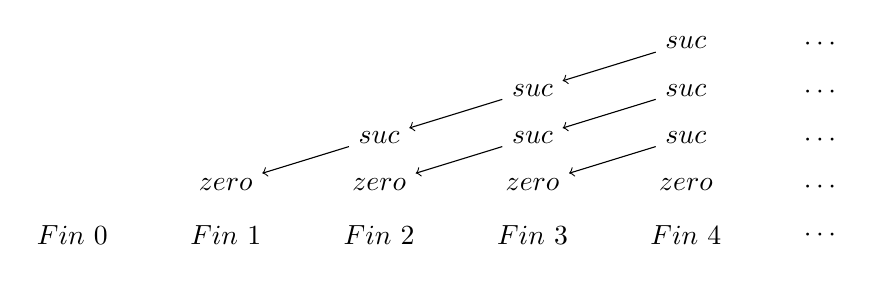
\begin{tikzpicture}[node distance=0.2cm and 0.8cm, auto]
  \node (fz) {$\Fin\ \lit{0}$};
  \node (fsz) [right=of fz] {$\Fin\ \lit{1}$};
  \node (fssz) [right=of fsz] {$\Fin\ \lit{2}$};
  \node (fsssz) [right=of fssz] {$\Fin\ \lit{3}$};
  \node (fssssz) [right=of fsssz] {$\Fin\ \lit{4}$};
  \node (fsssssz) [right=of fssssz] {$\cdots$};
  \node (z1) [above=of fsz] {$\zero$};
  \node (z2) [above=of fssz] {$\zero$};
  \node (z3) [above=of fsssz] {$\zero$};
  \node (z4) [above=of fssssz] {$\zero$};
  \node (z5) [above=of fsssssz] {$\cdots$};
  \node (sz2) [above=of z2] {$\suc$};
  \node (sz3) [above=of z3] {$\suc$};
  \node (sz4) [above=of z4] {$\suc$};
  \node (sz5) [above=of z5] {$\cdots$};
  \node (ssz3) [above=of sz3] {$\suc$};
  \node (ssz4) [above=of sz4] {$\suc$};
  \node (ssz5) [above=of sz5] {$\cdots$};
  \node (sssz4) [above=of ssz4] {$\suc$};
  \node (sssz5) [above=of ssz5] {$\cdots$};
  \draw[->] (sz2) to (z1);
  \draw[->] (sz3) to (z2);
  \draw[->] (sz4) to (z3);
  \draw[->] (ssz3) to (sz2);
  \draw[->] (ssz4) to (sz3);
  \draw[->] (sssz4) to (ssz3);
\end{tikzpicture}
\caption{We can visualize the family of $\Fin$ types as an (infinite) triangle,
where each type other than $\Fin\ \lit{0}$ has an element $\zero$, and each type also
has all elements of the form $\suc\ x$ where $x$ belongs to the \emph{previous}
type in the family.}
\end{figure}


%  \draw[-] (w) to node[above]{$t$} (x);
%  \draw[-] (y) to node[below]{$b$} (z);
%  \draw[-] (w) to node[left]{$l$} (y);
%  \draw[-] (x) to node[right]{$r$} (z);
%  \draw[-,double distance=3] (t) to node[right]{$q$} (b);

For now, let us define a safe variant of the $\fun{lookup}$ function
using $\Vec$ and $\Fin$. Here is the type signature:
\begin{code}[hide]
module LookupVec1 where
\end{code}
\begin{code}[number]
  lookupVec : {A : Set} {n : Nat} → Vec A n → Fin n → A
  lookupVec xs i = {!!}
\end{code}
Notice that the length $n$ of the vector is also used as the upper
bound for the position: this way we enforce that the position really is in
range of the vector. We then split on the vector $\var{xs}$ using \texttt{Ctrl+c Ctrl+c}:
\begin{code}[hide]
module LookupVec2 where
\end{code}
\begin{code}[number]
  lookupVec : {A : Set} {n : Nat} → Vec A n → Fin n → A
  lookupVec []         i = {!!}
  lookupVec (x :: xs)  i = {!!}
\end{code}
So far, so good. Next, we split on the position $i$ in the
first clause:
\begin{code}[hide]
module LookupVec3 where
\end{code}
\begin{code}[number]
  lookupVec : {A : Set} {n : Nat} → Vec A n → Fin n → A
  lookupVec []         ()
  lookupVec (x :: xs)  i   = {!!}
\end{code}
Something interesting has happened: the position has been replaced by
the special syntax $()$ and the equality sign
has disappeared. This is Agda's way to indicate that there is no
element of type $\Fin\ \zero$, i.e.~there is no possible position in a
vector of length $\lit{0}$. The special pattern $()$ used to indicate this
is called an \emph{absurd pattern}, and the clause is called an
\emph{absurd clause}.


Having completed the case for the empty vector $\nil$, we can
also split on the position $i$ in the second clause:
\begin{code}[hide]
module LookupVec4 where
\end{code}
\begin{code}[number]
  lookupVec : {A : Set} {n : Nat} → Vec A n → Fin n → A
  lookupVec []         ()
  lookupVec (x :: xs)  zero     = {!!}
  lookupVec (x :: xs)  (suc i)  = {!!}
\end{code}
Since the length of the vector $x\ \cons\ \var{xs}$ is $\suc\ n$,
we get cases for both constructors of $\Fin$.
Finally, we can complete the definition of $\fun{lookupVec}$ by
filling in the remaining two holes the same way as we would have done
for the unsafe lookup function in Haskell.
\begin{code}[number]
lookupVec : {A : Set} {n : Nat} → Vec A n → Fin n → A
lookupVec []         ()
lookupVec (x :: xs)  zero     = x
lookupVec (x :: xs)  (suc i)  = lookupVec xs i
\end{code}
Thanks to the power of dependent types, we have managed to implement a
\emph{safe} and \emph{total} version of the lookup function, without
having to change the return type in any way.

\marginnote{
\begin{exercise}
Implement a function $\fun{putVec} : \{ A : \ty{}
\} \{ n : \Nat \} \to \Fin\ n \to A \to \Vec\ A\ n \to \Vec\ A\ n$ that
sets the value at the given position in the vector to the given value,
and leaves the rest of the vector unchanged.
\end{exercise}
}

\subsection{The dependent pair type}

Another important type for programming with dependent types is called
the $\Sigma$ type or the \emph{dependent pair
type}. It can be seen as a generalization of the normal pair type
$A\ \prod\ B$ where the type of the second component can be different
depending on the value of the first component. For example, the type
$\sigmatype\ \Nat\ (\Vec\ \Bool)$ (or equivalently,
$\sigmatype\ \Nat\ (\lambda n \to \Vec\ \Bool \ n)$) contains the
elements $\lit{2}\ \con{,}\ (\true\ \cons\ \false\ \cons\ \nil)$ and
$\lit{0}\ \con{,}\ \nil$ but not $\lit{2}\ \con{,}\ \nil$ (since $\nil$ does not
have type $\Vec\ \Bool\ \lit{2}$). In general, this type consists of pairs
$m\ \con{,}\ \var{xs}$ where $m : \Nat$ and $\var{xs} : \Vec\ A\ m$.%
\footnote{The dependent pair type is also called the $\Sigma$ type
because it can be seen as a \emph{sum} (or disjoint union) of all
the types $B\ x$, where we view the first component as a label indicating
which type of the family the second component belongs to.}

We can define the type $\sigmatype$ of dependent pairs as follows:%
\footnote{To write $\Sigma$, type \texttt{\textbackslash{}Sigma}.}
\begin{code}[number]
data Σ (A : Set) (B : A → Set) : Set where
  _,_ : (x : A) → B x → Σ A B
\end{code}
Note that the second parameter of $\sigmatype$ is not just a type in
$\ty{}$ but a \emph{function} of type $A → \ty{}$, i.e.~a dependent type.

We can see that $\sigmatype$ is indeed a generalization of the normal
pair type where the type of the second component ignores its input:%
\footnote{This definition defines $A\ \data{×'}\ B$ to be a \emph{type alias}
for $\sigmatype~A~(λ\_ → B)$.}
\begin{code}[number]
_×'_ : (A B : Set) → Set
A ×' B = Σ A (λ _ → B)
\end{code}
\marginnote{
\begin{exercise}
Implement functions converting back and forth
between $A\ \prod\ B$ and $A\ \data{×'}\ B$.
\end{exercise}
}
We have the following functions for getting the individual components
of a dependent pair:
\begin{code}[number]
fstΣ : {A : Set}{B : A → Set} → Σ A B → A
fstΣ (x , y) = x

sndΣ : {A : Set}{B : A → Set} → (z : Σ A B) → B (fstΣ z)
sndΣ (x , y) = y
\end{code}
Note that return type of $\fun{sndΣ}$ depends on the result of the
first component $\fun{fstΣ}$.

An important use of the $\sigmatype$ type is to \emph{hide} some of
the information in a type when it is not relevant. For example, we can
hide the length of a vector by pairing it up with its length:
\begin{code}[number]
List' : (A : Set) → Set
List' A = Σ Nat (Vec A)
\end{code}
\marginnote{
\begin{exercise}
Implement functions converting back and forth
between $\List\ A$ and $\data{List'}\ A$.
\end{exercise}
}

\subsection{Section summary}

\begin{itemize}
  \item A dependent type is a family of types that is indexed over
values of a base type. For example, $\Vec\ A\ n$ is a dependent type
indexed over natural numbers $n : \Nat$.
  \item A dependent function is a function where the type of the
output depends on the value of the input. For example, $\fun{zeroes} :
(n : \Nat) \to \data{Vec}\ \Nat\ n$ is a dependent function.
  \item We can define new dependent types as \emph{indexed datatypes},
which are datatypes of type $I \to \ty{}$. Each constructor of an
indexed datatype must determine what index it targets. For example,
the constructor $\nil$ targets the type $\data{Vec}\ A\ \lit{0}$ with
index $\lit{0}$.
  \item When pattern matching on an indexed datatype, it is allowed to
omit constructors that can be determined to be impossible based on
their type. For example, the function $\fun{head}$ takes an argument
of type $\data{Vec}\ A\ (\suc\ n)$ so it does not require a case for
the empty vector $\nil$.
  \item When a type has no possible constructors, we can match on it
by using an \emph{absurd pattern} $()$ and omitting the right-hand
side of the clause.
  \item The dependent pair type $\sigmatype\ A\ B$ consists of pairs
$(x,y)$ where $x : A$ and $y : B\ x$.
\end{itemize}

\section{The Curry-Howard correspondence}


Now as we said before, Agda is not just a programming language but
also a proof assistant. This means we can use Agda to formulate
theorems and prove them, and Agda will check that the proofs are
correct. However, before we can use Agda as a proof assistant, we
first have to take a step back and understand the connection between
type systems and mathematical logic. This connection is known as the
\emph{Curry-Howard correspondence}, named so after the mathematician
Haskell B.~Curry (yes, that one), who discovered the correspondence
between a simple type system and propositional logic in 1934, and the
logician William A.~Howard, who extended the isomorphism to
quantifiers such as $\forall$ (`for all') and $\exists$ (`exists') in
1969.

The core idea of the Curry-Howard correspondence is that we can
interpret logical propositions --- such as ``$P$ and $Q$'', ``not $P$'',
``$P$ implies $Q$'', \ldots --- as \emph{types} whose elements are valid
proofs of that proposition.

\subsection{Propositional logic}

To get a better idea of what this means, we will take a look at
several logical propositions and deduce what type they correspond
to. For each proposition, we ask two important questions: how do we
\emph{prove} this proposition, and what can we \emph{deduce} from it?

\begin{description}

\item[Conjunction.] As a first example, consider the proposition ``$P$
and $Q$''. What do we need in order to prove it? Well, we first need a
proof of $P$, and we also need a proof of $Q$. Hence a proof of ``$P$
and $Q$'' is a \emph{pair} $(p,q)$ of two proofs, where $p$ is a proof
of $P$ and $q$ is a proof of $Q$.  Similarly, if we are working on a
proof and have an assumption that ``$P$ and $Q$'' holds, then we can
deduce that both $P$ holds and $Q$ holds. So given a proof $r$ of
``$P$ and $Q$'', we can get a proof $\fun{fst}\ r$ of $P$ and another
proof $\fun{snd}\ r$ of $Q$. So under the Curry-Howard correspondence,
``$P$ and $Q$'' corresponds to the pair type $P\ \prod\ Q$.

\item[Implication.] As a second example, let's look at the proposition
``$P$ implies $Q$''. In order to prove this implication, we may assume
that we have a proof $x$ of $P$ holds and from that we need to
construct a proof $q$ of $Q$. In other words, a proof of ``$P$ implies
$Q$'' is a \emph{function} $\lambda\ x \to q$ that transforms a proof
of $P$ into a proof of $Q$. In addition, if we have both a proof $f$
of ``$P$ implies $Q$'' and a proof $p$ of $P$, then we can combine the
two proofs to get a new proof $f\ p$ of $Q$. So under the Curry-Howard
correspondence, ``$P$ implies $Q$ corresponds to the function type $P
\to Q$.

\item[Disjunction.] What type corresponds to the proposition ``$P$ or
$Q$''? In order to prove it, we need to either provide a proof $p$ of
$P$ or a proof $q$ of $Q$. To avoid confusion between whether we
proved $P$ or $Q$, we can label the proofs as either $\con{left}\ p$
or $\con{right}\ q$. Using a proof of ``$P$ or $Q$'' is a bit less
straightforward. If we know that $P$ holds or $Q$ holds and we want to
prove $R$, then we need to show two things: (1) that $P$ implies $R$,
and (2) that $Q$ implies $R$. We can summarize this proof of $R$ as
$\fun{cases}\ z\ f\ g$ where $z$ is a proof of ``$P$ or $Q$'', $f$ is
a proof of ``$P$ implies $R$'', and $g$ is a proof of ``$Q$ implies
$R$'' (i.e.~$f : P \to R$ and $g : Q \to R$). In conclusion, the
proposition ``$P$ or $Q$'' corresponds to the type $\data{Either}\ P\
Q$ under the Curry-Howard correspondence.

\marginnote{
\begin{exercise}
Define the $\data{Either}$ type in Agda, and write
down a definition of the function $\fun{cases} : \{ A\ B\ C : \ty{} \}
\to \data{Either}\ A\ B \to (A \to C) \to (B \to C) \to C$.
\end{exercise}
}

\begin{code}[hide]
data Either (A B : Set) : Set where
  left   : A → Either A B
  right  : B → Either A B

cases : {A B C : Set} → Either A B → (A → C) → (B → C) → C
cases (left x)   f  g  = f x
cases (right y)  f  g  = g y
\end{code}

\item[Truth.] A very basic proposition is ``\emph{true}'', i.e.~the
proposition that always holds no matter what. Proving it is
straightforward: we don't need to provide any assumptions. We could
thus say there is a trivial proof $\con{tt}$ of ``\emph{true}''. On
the other hand, assuming ``\emph{true}'' in a proof does not provide
any new information. We can thus say that ``\emph{true}'' corresponds
to the unit type $\toptype$\footnote{Unicode input for $\top$ is
\texttt{\textbackslash{}top}.}, which is defined as follows:
\begin{code}[number]
data ⊤ : Set where
  tt : ⊤
\end{code}
(This is very similar to the empty tuple type \texttt{()} in Haskell,
which has a single inhabitant \texttt{() :: ()}.)

\item[Falsity.] The other basic proposition is ``\emph{false}'', the
proposition that is never true.
There are no ways to prove it, which
suggests that it should correspond to an \emph{empty} type. In Agda,
we can define the empty type $\bottomtype$\footnote{Unicode input for
$\bot$ is \texttt{\textbackslash{}bot}.} as a datatype with no
constructors:
\begin{code}[number]
data ⊥ : Set where
  -- no constructors
\end{code}
On the other hand, if we assume we have a proof $p$ of
``\emph{false}'', then the principle of explosion (also known under
the latin name ``ex falso quodlibet'', or ``from falsity follows
anything'') tells us we can can get a proof $\fun{absurd}\ p$ of any
proposition we want. In Agda, we can define $\fun{absurd}$ as follows:
\begin{code}[number]
absurd : {A : Set} → ⊥ → A
absurd ()
\end{code}
(Remember that the absurd pattern $()$ indicates to Agda that there
are no valid constructors.)
\marginnote[-4cm]{%
\paragraph{On empty types.} Note that it is not possible to
define a real empty type in Haskell: even if we define a type with no
constructors, it is still inhabited by \texttt{undefined}, as well as
infinitely looping programs. So in order to express false
propositions, it is essential to work in a total language such as
Agda.}
\end{description}


\marginnote[-1cm]{%
\paragraph{Propositional logic versus boolean logic.} On the
surface, the two types $\toptype$ and $\bottomtype$ seem to be very
similar to the booleans $\true$ and $\false$. However, they have a
very different role: $\true$ and $\false$ are \emph{values} that our
Agda programs can manipulate and return, while $\toptype$ and
$\bottomtype$ are \emph{types} used by Agda itself. In particular, it
is not possible to write a program to check whether a given type is
$\toptype$ or $\bottomtype$. So think carefully which one you want to
use in what situation!
}

From these basic propositions, we can derive some other notions:
\begin{description}
\item[Negation.] We can encode ``not $P$'' as the type $P \to \bottomtype$.

\item[Equivalence.] We can encode ``$P$ is equivalent to $Q$'' as $(P
\to Q) \prod (Q \to P)$.  \end{description} The correspondences
between propositions and types we have discussed so far are summarized
in Table~\ref{tab:curry-howard-simple}.

\begin{table}[ht]
\centering
\fontfamily{ppl}\selectfont
\begin{tabular}{r>{\columncolor{gray!30}}cl}
\textbf{Propositional logic} & & \textbf{Type system} \\
proposition & $P$ & type \\
proof of a proposition & $p : P$ & program of a type \\
conjunction & $P\ \prod\ Q$ & pair type \\
disjunction & $\data{Either}\ P\ Q$ & either type \\
implication & $P \rightarrow Q$ & function type \\
truth & $\toptype$ & unit type \\
falsity & $\bottomtype$ & empty type \\
negation & $P \rightarrow \bot$ & function to $\bot$ \\
equivalence & $(P \rightarrow Q)\ \prod\ (Q \rightarrow P)$ & pair of two functions \\
\end{tabular}
\label{tab:curry-howard-simple}
\caption{The Curry-Howard correspondence between propositional logic and simple (non-dependent) types in Agda.}
\end{table}

Thanks to the Curry-Howard correspondence, we can take any formula in
propositional logic, translate it to a type in Agda, and then
\emph{prove} the formula by writing down a function of that
type. Let's look at some examples:
\begin{itemize}

\item The proposition ``$P$ implies $P$'' translates to the Agda type
$P \to P$, which we can prove as follows:
\begin{code}[number]
proof1 : {P : Set} → P → P
proof1 p = p
\end{code}
Note that this is simply the identity function $\fun{id}$.

\item The proposition ``If ($P$ implies $Q$) and ($Q$ implies $R$)
then ($P$ implies $R$)'' translates to the Agda type $(P \to Q)\
\prod\ (Q \to R) \to (P \to R)$, which we can prove as follows:
\begin{code}[number]
proof2 : {P Q R : Set} → (P → Q) × (Q → R) → (P → R)
proof2 (f , g) = λ x → g (f x)
\end{code}
Note that this is exactly (the uncurried version of) function composition.

\item The proposition ``If ($P$ or $Q$) implies $R$ then ($P$ implies
$R$) and ($Q$ implies $R$)'' translates to the Agda type
$(\data{Either}\ P\ Q \to R) \to (P \to R)\ \prod\ (Q \to R)$, which
we can prove as follows:
\begin{code}[number]
proof3 : {P Q R : Set}
       → (Either P Q → R) → (P → R) × (Q → R)
proof3 f = (λ x → f (left x)) , (λ y → f (right y))
\end{code}

\end{itemize}

\marginnote[-13cm]{
\begin{exercise}
Translate the following propositions to Agda types
using the Curry-Howard correspondence, and prove them by implementing
a function of that type.
\begin{itemize}
\item If $A$ then ($B$ implies $A$).
\item If ($A$ and \emph{true}) then ($A$ or \emph{false}).
\item If $A$ implies ($B$ implies $C$), then ($A$ and $B$) implies $C$.
\item If $A$ and ($B$ or $C$), then either ($A$ and $B$) or ($A$ and $C$).
\item If $A$ implies $C$ and $B$ implies $D$, then ($A$ and $B$) implies ($C$ and $D$).
\end{itemize}
\end{exercise}
}


\marginnote[-8cm]{
\paragraph{Constructive mathematics.}
You may already have noticed that certain propositions that are
typically held to be true cannot be proven when translated to Agda via
the Curry-Howard correspondence. For example, the law of the excluded
middle (``either $P$ or not $P$'') translates to the type $\{ P :
\ty{} \} \to \data{Either}\ P\ (P \to \bottomtype)$, for which we
cannot in general provide an implementation without knowing anything
about $P$. The reason is that Agda uses a \emph{constructive logic},
as opposed to the classical logic typically used in mathematics. In
particular, a constructive proof of ``$P$ or $Q$'' requires us to have
a decision procedure to determine whether $P$ holds or $Q$
holds. While this seems like a major limitation of Agda, experience
shows it is only very rarely a problem in practice: most of the time a
proof that uses the excluded middle can be rewritten in a way such
that it doesn't.

For the rare cases where you want to prove a proposition that only
holds in classical logic, it is possible to translate between
constructive and classical logic using the \emph{double negation
translation}: a proposition $P$ is true in classical logic if and only
if ``not (not $P$)'' is true in constructive logic. So to prove a
proposition $P$ using classical logic, all we have to do is prove $(P
\to \bottomtype) \to \bottomtype$ in the constructive logic of Agda.
}

\marginnote{
\begin{exercise}
Write a function of type $\{ P : \ty{} \} \to
(\data{Either}\ P\ (P \to \bottomtype) \to \bottomtype) \to
\bottomtype$.
\end{exercise}
}

\subsection{Predicate logic}

So far, we have used the Curry-Howard correspondence to view formulas
from propositional logic as Agda types, and prove them by writing down
functions. However, we would also like to write down and prove
propositions that say something about a given value or function. For
example, we would like to be able to prove that $\lit{6}$ is even, or that
$\fun{length}\ (\fun{map}\ f\ \var{xs})$ is equal to $\fun{length}\
\var{xs}$ for all $\var{xs}$, or that there exists a number $n$ such
that $n\ \fun{+}\ n = \lit{12}$. In order to prove such statements, we first
need to answer two more questions: how can we define predicates that
express concrete properties such as being even, and how can we express
quantifiers such as ``for all'' and ``there exists''.

Let's start with the first question. Since --- according to Curry-Howard
--- propositions are types, we can define new propositions by defining
new data types. For example, we can define a type $\fun{IsEven}\ n$ that
expresses whether $n$ is even by pattern matching on $n$:
\begin{code}[number]
data IsEven : Nat → Set where
  even-zero : IsEven zero
  even-suc2 : {n : Nat} → IsEven n → IsEven (suc (suc n))
\end{code}
Note that $\data{IsEven}$ is an \emph{indexed datatype}, just like
$\data{Vec}$ and $\data{Fin}$ We can then easily prove that $\lit{6}$ is
even:
\begin{code}[number]
6-is-even : IsEven 6
6-is-even = even-suc2 (even-suc2 (even-suc2 even-zero))
\end{code}
On the other hand, there is no way to prove that $\lit{7}$ is even:
$\data{IsEven}\ \lit{7}$ is an empty type. In fact, we can prove that
$\data{IsEven}\ \lit{7}$ is false by defining a function from this type to
$\bottomtype$:
\begin{code}[number]
7-is-not-even : IsEven 7 → ⊥
7-is-not-even (even-suc2 (even-suc2 (even-suc2 ())))
\end{code}
Here we have to case split four times (using \texttt{Ctrl+c Ctrl+c})
before Agda can see that there is indeed no proof of
$\data{IsEven}\ \lit{7}$. Note in particular that it is possible for a
absurd pattern $()$ to appear as an argument to a constructor.

One predicate that is often quite useful is the predicate stating that
a given $\Bool$ is $\true$. It can be defined as follows:
\begin{code}[number]
data IsTrue : Bool → Set where
  is-true : IsTrue true
\end{code}
\marginnote{
\paragraph{Defining properties as functions.}
In this section we define new properties as
Agda data types. An alternative approach is to define new properties
as \emph{functions} that return a value of type $\ty{}$. For example,
an alternative definition of $\data{IsTrue}$ could be given as:
\begin{code}[number]
IsTrue' : Bool → Set
IsTrue' true   = ⊤
IsTrue' false  = ⊥
\end{code}
This approach often results in proofs that are shorter, but less readable.  It
is also less general, as some types (such as the identity type which
we will discuss in the next section) can only be defined as a data
type. Hence we prefer the approach using data types over the one using
functions.
}
The type $\data{IsTrue}\ b$ has exactly one constructor if and only if
$b$ is $\true$, and it is empty if $b$ is false. By using this type in
conjunction with a function that returns a boolean, we can easily
express many properties. For example, we can define the function
$\fun{\_=Nat\_}$ that checks equality of two numbers,\footnote{Note that
$\Nat$ is just a user-defined datatype in Agda, so it does not come with
a predefined notion of equality.}
and use it to
prove that the list $\lit{1}\ \cons\ \lit{2}\ \cons\ \lit{3}\ \cons\
\nil$ has length $\lit{3}$:
\begin{code}[number]
_=Nat_ : Nat → Nat → Bool
zero     =Nat  zero     = true
(suc x)  =Nat  (suc y)  = x =Nat y
_        =Nat  _        = false

length-is-3 : IsTrue (length (1 :: 2 :: 3 :: []) =Nat 3)
length-is-3 = is-true
\end{code}


\subsection{Universal and existential quantifiers}

Next, we would like to express properties that quantify over a given
type, using quantifiers such as $\forall$ (``for all'') and $\exists$
(``there exists''). Luckily, we already have all the types we need, we
just didn't realize it yet!

\begin{description}

\item[Universal quantification] Consider the proposition ``for all $x$
of type $A$, $P(x)$''. To prove it, we need to be able to provide a
proof of $P(v)$ for each concrete value $v : A$. In other words, we
need a \emph{function} $\lambda v → p$ that for each $v$ produces a
proof $p$ of $P(v)$. In the opposite direction, if we assume we have a
proof $f$ of ``for all $x$ of type $A$, $P(x)$'' and we have a
concrete value $v : A$, then we can apply the proof to the case of $v$
to get a proof $f\ v$ of $P(v)$. So under the Curry-Howard
correspondence, ``for all $x$ of type $A$, $P(x)$'' corresponds to the
\emph{dependent function type} $(x : A) → P\ x$.

\item[Existential quantification] Next, consider the proposition
``there exists a $x : A$ such that $P(x)$''. To prove it, we need to
provide a concrete example $v : A$, and provide a proof $p$ that
$P(v)$ holds, i.e. we need a \emph{pair} $(v,p)$ of a $v : A$ and a $p
: P\ v$. Conversely, if we have a proof $z$ of ``there exists a $x :
A$ such that $P(x)$'' then we should be able to extract the witness
$\fun{fst}\ z : A$ as well as the proof $\fun{snd}\ z : P\ (\fun{fst}\
z)$. From this we deduce that ``there exists a $x : A$ such that
$P(x)$'' corresponds to the \emph{dependent pair type} $\sigmatype\ A\
(\lambda\ x \to P\ x)$.

\end{description}

We extend the table summarizing the Curry-Howard correspondence with
universal and existential quantification in
Table~\ref{tab:curry-howard-full}.

\begin{table}
\begin{tabular}{r>{\columncolor{gray!30}}cl}
\textbf{Propositional logic} & & \textbf{Type system} \\
proposition & $P$ & type \\
proof of a proposition & $p : P$ & program of a type \\
conjunction & $P\ \prod\ Q$ & pair type \\
disjunction & $\data{Either}\ P\ Q$ & either type \\
implication & $P \rightarrow Q$ & function type \\
truth & $\toptype$ & unit type \\
falsity & $\bottomtype$ & empty type \\
negation & $P \rightarrow \bot$ & function to $\bot$ \\
equivalence & $(P \rightarrow Q)\ \prod\ (Q \rightarrow P)$ & pair of two functions \\
universal quantification & $(x : A) → P\ x$ & dependent function type \\
existential quantification  & $\sigmatype\ A\ (\lambda\ x → P\ x)$ & dependent pair type \\
\end{tabular}
\label{tab:curry-howard-full}
\caption{The Curry-Howard correspondence between predicate logic and dependent types in Agda.}
\end{table}

As an example, we can prove that for any natural number $n$,
$\fun{double}\ n$ is even:
\begin{code}[number]
double : Nat → Nat
double zero     = zero
double (suc n)  = suc (suc (double n))

double-is-even : (n : Nat) → IsEven (double n)
double-is-even zero     = even-zero
double-is-even (suc m)  = even-suc2 (double-is-even m)
\end{code}
Let's take a closer look at the implementation of
$\fun{double-is-even}$. It makes use of two features we've used
before: \emph{pattern matching} and \emph{recursion}. Through the lens
of the Curry-Howard correspondence, we can see these two features in a
new light.
\begin{itemize}

\item By pattern matching on the natural number $n$, we are doing a
\emph{proof by cases} on $n$, which allows us to prove the cases $n =
\zero$ and $n = \suc\ m$ separately. Thanks to Agda's coverage
checker, we can be sure that the proof covers all cases.

\item By making a recursive call to $\fun{double-is-even}\ m$ on the
right-hand side for $\fun{double-is-even}\ (\suc\ m)$, we are making
use of \emph{induction} on the number $n$: we assume that the
proposition holds for $n = m$, and from that we prove that it holds
for $n = \suc\ m$. By induction, we can then conclude that it holds
for all values of $n$. Thanks to Agda's termination checker, we can be
sure that we only make use of the inductive hypothesis for smaller
values of $n$.

\end{itemize}
So in summary, thanks to the Curry-Howard correspondence we can use
familiar techniques from functional programming to write formal
proofs!

As another example, we can prove that for any number $n$, $n\
\fun{=Nat}\ n$ is $\true$:
\begin{code}[number]
n-equals-n : (n : Nat) → IsTrue (n =Nat n)
n-equals-n zero     = is-true
n-equals-n (suc m)  = n-equals-n m
\end{code}

We can now also prove existential statements by making use of the
$\sigmatype$ type. For example, we can prove that there exists a
number $n$ such that $n\ \fun{+}\ n = \lit{12}$ by exhibiting the number
$\lit{6}$:
\begin{code}[number]
half-a-dozen : Σ Nat (λ n → IsTrue ((n + n) =Nat 12))
half-a-dozen = 6 , is-true
\end{code}


As another example, we can prove that any number $n$ is either $\lit{0}$ or
the successor of another number $m$:
\begin{code}[number]
zero-or-suc : (n : Nat)
  → Either (IsTrue (n =Nat 0))
           (Σ Nat (λ m → IsTrue (n =Nat (suc m))))
zero-or-suc zero     = left is-true
zero-or-suc (suc m)  = right (m , n-equals-n m)
\end{code}

\subsection{The identity type}

In the previous section, we proved that \texttt{length (xs ++ ys)} is
equal to \texttt{length xs + length ys} by making use of the function
$\fun{\_=Nat\_}$ together with the predicate $\fun{IsTrue}$. This
method works for concrete types such as natural numbers, but it has a
fundamental flaw: if we want to prove something about a function with
return type $X$, we first need to define a function $\fun{\_=X\_} : X
\to X \to \Bool$. This can be rather difficult, and moreover it
doesn't work for abstract type variables: how would we state that
$\fun{id}\ x$ is equal to $x$ for variables $x : A$ of \emph{any} type
$A$?

In order to express equality at any type, Martin-L\"of introduced a
new type $x\ \Id\ y$\footnote{Unicode input for $\equiv$ is
\texttt{\textbackslash{}equiv}.}, called the \emph{identity type},%
\footnote{Do not confuse the \emph{identity type} $x\ \Id\ y$ with the
(type of the) \emph{identity function} $\fun{id} : \{A:\ty{}\} \to A
\to A$.}  with a single constructor $\refl : x\ \Id\ x$ (short for
`reflexivity'). If $x$ and $y$ are equal, then $x\ \Id\ y$ has a
single inhabitant $\refl$, so it behaves like the unit type
$\toptype$.  On the other hand, if $x$ and $y$ are distinct (e.g.~$x =
\zero$ and $y = \suc\ \zero$) then $x\ \Id\ y$ has no constructors and
hence it behaves like the empty type $\bottomtype$.  In Agda, we can
define the identity type as follows:
\begin{code}[number]
data _≡_ {A : Set} : A → A → Set where
  refl : {x : A} → x ≡ x

infix 4 _≡_
\end{code}
Just like $\Vec$ and $\data{Even}$, $\data{\_≡\_}$ is defined as an
indexed datatype, this time with two indices of type $A$.

With this type, we can for example prove that, indeed,
$1+1=2$:\footnote{\thepage{} pages is still better than the 362 pages
that Whitehead and Russell needed to prove this fact!}
\begin{code}[number]
one-plus-one : 1 + 1 ≡ 2
one-plus-one = refl
\end{code}
\ldots and that $\lit{0}$ is not equal to $\lit{1}$:\footnote{Exciting!}
\begin{code}[number]
zero-not-one : 0 ≡ 1 → ⊥
zero-not-one ()
\end{code}
We can also prove facts about polymorphic types, for example that the
$\fun{id}$ function always returns its input:
\begin{code}[number]
id-returns-input : {A : Set} → (x : A) → id x ≡ x
id-returns-input x = refl
\end{code}

\marginnote{
\paragraph{Unit tests in Agda.} A neat trick you can do in
Agda is to write unit tests directly in your code by making use of the
identity type. For example, we can write a test that $\fun{length}\
(\lit{1}\ \cons\ \lit{2}\ \cons\ \nil)$ is $\lit{2}$ as follows:
\begin{code}[number]
length-test1 :
  length (1 :: 2 :: []) ≡ 2
length-test1 = refl
\end{code}
When the Agda typechecker checks that $\refl : \fun{length}\ (\lit{1}\
\cons\ \lit{2}\ \cons\ \nil)\ \Id\ \lit{2}$, it will evaluate both sides
to make sure they are indeed equal. So if anything changes and the
test no longer succeeds, you will know immediately as the file will
not even typecheck any more!
}

Despite the fact that the identity type only has a single inhabitant
$\refl$, we can prove other properties of equality: symmetry (if
$x=y$, then $y=x$), transitivity (if $x=y$ and $y=z$ then $x=z$), and
congruence (if $x=y$ then $f(x)=f(y)$). To prove these properties, we
have to match on an argument of type $x\ \Id\ y$. Since $\refl$ is the
only constructor of this type, there is always only a single
case. However, pattern matching on $\refl$ is not useless: by matching
a proof of $x\ \Id\ y$ against the constructor $\refl$, Agda learns
that $x$ and $y$ are indeed equal. For example, in the definition of
$\fun{sym}$ below, matching on $\refl$ teaches Agda that $x$ and $y$
must be equal, which is required for the right-hand side $\refl$ to be
accepted at type $y\ \Id\ x$.

\begin{code}[number]
-- symmetry of equality
sym : {A : Set} {x y : A} → x ≡ y → y ≡ x
sym refl = refl

-- transitivity of equality
trans : {A : Set} {x y z : A} → x ≡ y → y ≡ z → x ≡ z
trans refl refl = refl

-- congruence of equality
cong : {A B : Set} {x y : A} → (f : A → B) → x ≡ y → f x ≡ f y
cong f refl = refl
\end{code}

In general, there are two cases where we can match on a proof of $a\ \Id\ b$:
\begin{itemize}

\item If $a$ and $b$ can be unified by instantiating some of the
variables, then we can match on $\refl$.

\item If $a$ and $b$ are obviously different (e.g.~ are applications
of different constructors) then we can match on an absurd pattern $()$

\end{itemize}
In all other cases where $a$ and $b$ cannot easily be unified but they
are not obviously distinct either, Agda will throw an error message
saying it doesn't know whether there should be a case for the
constructor $\refl$.

\subsection{Section summary}

\begin{itemize}
  \item The Curry-Howard correspondence tells us that we can interpret
logical propositions as the types of valid proofs of that proposition.
  \item Under the Curry-Howard correspondence, conjunction $A \land B$
corresponds to the pair type $A\ \data{×}\ B$, implication $A
\Rightarrow B$ corresponds to the function type $A \to B$, disjunction
$A \lor B$ corresponds to the type $\data{Either}\ A\ B$, truth
corresponds to the unit type $\data{⊤}$, and falsity corresponds to
the empty type $\data{⊥}$.
\item Under the Curry-Howard correspondence, predicates on values
correspond to \emph{dependent types}. For example, we can represent
the predicate `$n$ is even' as the type $\data{IsEven}\ n$.
\item Universal quantification $\forall (x\in A).~P(x)$ corresponds to
the dependent function type $(x : A) → P\ x$, and existential
quantification $\exists (x\in A).~P(x)$ corresponds to the dependent
pair type $\sigmatype\ A\ (\lambda x → P\ x)$.
\item The identity type $x~\data{≡}~y$ represents the proposition that
$x$ and $y$ are equal. It is defined as an indexed datatype with a
single constructor $\con{refl} : x~\data{≡}~x$. Other properties of
equality such as symmetry, transitivity, and congruence can be proven
by pattern matching on $\refl$.
\end{itemize}

\section{Equational reasoning in Agda}

In chapter 16 of his book \emph{Programming in Haskell}, Hutton
explains how to use \emph{equational reasoning} to prove properties of
Haskell functions. However, these proofs quickly become long and
rather boring, which makes it easy for mistakes to slip through. In
Agda, we can do better: thanks to the Curry-Howard correspondence, we
can write proofs about Agda in Agda itself, and have the typechecker
check their correctness automatically. Moreover, thanks to Agda's
flexible operator syntax, we can even write these proofs in a style
very similar to Hutton's.

In order to write equational reasoning proofs in Agda, we first need
to define a few operators that will provide us with a nice syntax to
write down these proofs. It is normal that these definitions do not
make much sense on their own, but their usefulness will become
apparent soon.%
\footnote{To enter the $⟨$ symbol in Agda, write
\texttt{\textbackslash{}<}, and similarly for $\rangle$, write
\texttt{\textbackslash{}>}.}
\begin{code}[number]
begin_ : {A : Set} → {x y : A} → x ≡ y → x ≡ y
begin p = p

_end : {A : Set} → (x : A) → x ≡ x
x end = refl

_=⟨_⟩_ : {A : Set} → (x : A) → {y z : A}
       → x ≡ y → y ≡ z → x ≡ z
x =⟨ p ⟩ q = trans p q

_=⟨⟩_ : {A : Set} → (x : A) → {y : A} → x ≡ y → x ≡ y
x =⟨⟩ q = x =⟨ refl ⟩ q

infix   1  begin_
infix   3  _end
infixr  2  _=⟨_⟩_
infixr  2  _=⟨⟩_
\end{code}

\subsection{Simple examples}

As a first simple example of equational reasoning in Agda, let us
prove that $\fun{reverse}$ has no effect on singleton lists, in the
sense that $\fun{reverse}\ \fun{[}\ x\ \fun{]} = \fun{[}\ x\
\fun{]}$ for any value $x$, where $\fun{[}\ x\ \fun{]} = x\ \cons\
\nil$:
\begin{AgdaAlign}
\begin{AgdaSuppressSpace}
\begin{code}[number]
[_] : {A : Set} → A → List A
[ x ] = x :: []

reverse : {A : Set} → List A → List A
reverse [] = []
reverse (x :: xs) = reverse xs ++ [ x ]
\end{code}
\begin{code}[number]
reverse-singleton : {A : Set} (x : A) → reverse [ x ] ≡ [ x ]
reverse-singleton x =
  begin
    reverse [ x ]
  =⟨⟩                       --  definition of [_]
    reverse (x :: [])
  =⟨⟩                       --  applying reverse (second clause)
    reverse [] ++ [ x ]
  =⟨⟩                       --  applying reverse (first clause)
    [] ++ [ x ]
  =⟨⟩                       --  applying _++_
    [ x ]
  end
\end{code}
\end{AgdaSuppressSpace}
\end{AgdaAlign}
From this, we can see the general structure of a proof that uses
equational reasoning: it starts with $\fun{begin}$ and ends with
$\fun{end}$, and in between is a sequence of expressions separated by
$\fun{=⟨⟩}$ symbols. Each of the expressions should be equal to the
previous one, and the result of the whole block (starting with
$\fun{begin}$ and ending with $\fun{end}$) is a proof that the first
expression is equal to the last one. This results in proofs that are
very easy to read compared to ones using $\refl$ and $\fun{trans}$
directly.

\subsection{Proof by cases and induction}

We can combine equational reasoning with other techniques we have seen
before. For example, we can prove that $\fun{not}\ (\fun{not}\ b) = b$
by case analysis (i.e.~pattern matching) on $b$:
\begin{code}[number]
not-not : (b : Bool) → not (not b) ≡ b
not-not false =
  begin
    not (not false)
  =⟨⟩                -- applying the inner not
    not true
  =⟨⟩                -- applying not
    false
  end
\end{code}
\begin{code}[number]
not-not true =
  begin
    not (not true)
  =⟨⟩                -- applying the inner not
    not false
  =⟨⟩                -- applying not
    true
  end
\end{code}

We can also prove facts about natural numbers by induction
(i.e.~recursion). For example, we can prove that $n\ \fun{+}\ \lit{0} = n$
for all $n : \Nat$ (note that this fact is not immediately obvious
from the definition of $\fun{\_+\_}$, which only says something about
$\lit{0}\ \fun{+}\ n$ and $(\suc\ m)\ \fun{+}\ n$):
\begin{AgdaAlign}
\begin{AgdaSuppressSpace}
\begin{code}[number]
add-n-zero : (n : Nat) → n + zero ≡ n
add-n-zero zero =
  begin
    zero + zero
  =⟨⟩                             -- applying +
    zero
  end
\end{code}
\begin{code}[number]
add-n-zero (suc n) =
  begin
    (suc n) + zero
  =⟨⟩                             -- applying +
    suc (n + zero)
  =⟨ cong suc (add-n-zero n) ⟩    -- using induction hypothesis
    suc n
  end
\end{code}
\end{AgdaSuppressSpace}
\end{AgdaAlign}
In order to prove that $\suc\ (n\ \fun{+}\ \lit{0})$ is equal to $\suc\ n$,
we have to make use of the induction hypothesis $\fun{add-n-zero}\ n$,
which says that $n\ \fun{+}\ \lit{0} = n$. Agda cannot figure this out on its
own, so we have to provide the proof manually. This is where the
operator $\fun{\_=⟨\_⟩\_}$ comes in: it allows us to provide an
equality proof in between the angle brackets. We have to provide a
proof of $\suc\ (n\ \fun{+}\ \lit{0})\ \Id\ \suc\ n$ but $\fun{add-n-zero}\
n$ has type $n\ \fun{+}\ \lit{0}\ \Id\ n$, so we apply $\fun{cong}\ \suc$ to
it to apply $\suc$ to both sides of the equation.


\marginnote{
\begin{exercise}
Prove that $m\ \fun{+}\ \suc\ n = \suc\ (m\
\fun{+}\ n)$ for all natural numbers $m$ and $n$. Next, use the
previous lemma and this one to prove commutativity of addition,
i.e. that $m\ \fun{+}\ n = n\ \fun{+}\ m$ for all natural numbers $m$
and $n$.
\end{exercise}

\begin{code}[hide]
add-n-suc : (m n : Nat) → m + (suc n) ≡ suc (m + n)
add-n-suc zero    n =
  begin
    zero + (suc n)
  =⟨⟩                            -- applying +
    suc n
  end
add-n-suc (suc m) n =
  begin
    (suc m) + (suc n)
  =⟨⟩                            -- applying +
    suc (m + (suc n))
  =⟨ cong suc (add-n-suc m n) ⟩  -- using induction hypothesis
    suc (suc (m + n))
  end

add-comm : (m n : Nat) → n + m ≡ m + n
add-comm zero    n =
  begin
    n + zero
  =⟨ add-n-zero n ⟩              -- applying lemma add-n-zero
    n
  =⟨⟩                            -- unapplying add
    zero + n
  end
add-comm (suc m) n =
  begin
    n + (suc m)
  =⟨ add-n-suc n m ⟩             -- applying lemma add-n-suc
    suc (n + m)
  =⟨ cong suc (add-comm m n) ⟩   -- using induction hypothesis
    suc (m + n)
  =⟨⟩                            -- unapplying add
    (suc m) + n
  end
\end{code}

}

As another example, let us show that addition of natural numbers is
associative, i.e. that $x\ \fun{+}\ (y\ \fun{+}\ z) = (x\ \fun{+}\ y)\
\fun{+}\ z$. Since there are three variables, we have to choose on
which one to pattern match. Since $\fun{\_+\_}$ is defined by pattern
matching on its first argument, and $x$ appears twice as the first
argument to $\fun{\_+\_}$, it is natural to try matching on $x$ first:
\begin{AgdaAlign}
\begin{AgdaSuppressSpace}
\begin{code}[number]
add-assoc : (x y z : Nat) → x + (y + z) ≡ (x + y) + z
add-assoc zero y z =
  begin
    zero + (y + z)
  =⟨⟩                              -- applying the outer +
    y + z
  =⟨⟩                              -- unapplying add
    (zero + y) + z
  end
\end{code}
\begin{code}[number]
add-assoc (suc x) y z =
  begin
    (suc x) + (y + z)
  =⟨⟩                              -- applying the outer add
    suc (x + (y + z))
  =⟨ cong suc (add-assoc x y z) ⟩  -- using induction hypothesis
    suc ((x + y) + z)
  =⟨⟩                              -- unapplying the outer add
    (suc (x + y)) + z
  =⟨⟩                              -- unapplying the inner add
    ((suc x) + y) + z
  end
\end{code}
\end{AgdaSuppressSpace}
\end{AgdaAlign}

In general, each case of a proof typically starts by applying some
definitions, then perhaps applying an auxiliary lemma and/or induction
hypothesis, and finally unapplying some definitions. When you are
stuck writing a proof, it often helps to work from both directions:
`forwards' from the starting point and `backwards' from the final
result, until it becomes clear what step is still required.



\marginnote{
\begin{exercise}
Consider the following function:
\begin{code}[number]
replicate : {A : Set}
  → Nat → A → List A
replicate zero     x  = []
replicate (suc n)  x  =
  x :: replicate n x
\end{code}
Prove that the length of $\fun{replicate}\ n\ x$ is always equal to
$n$, by induction on the number $n$.
\end{exercise}
}

\begin{code}[hide]
length-replicate : {A : Set} → (n : Nat) (x : A) → length (replicate n x) ≡ n
length-replicate {A} zero x =
  begin
    length (replicate zero x)
  =⟨⟩                          -- applying replicate
    length {A} []
  =⟨⟩                          -- applying length
    zero
  end
length-replicate (suc n) x =
  begin
    length (replicate (suc n) x)
  =⟨⟩                              -- applying replicate
    length (x :: replicate n x)
  =⟨⟩                              -- applying length
    suc (length (replicate n x))
  =⟨ cong suc (length-replicate n x) ⟩  -- using induction hypothesis
    suc n
  end
\end{code}

\subsection{Induction on lists}

Induction can be used to prove properties of any recursive datatype,
not just natural numbers. As an example, we will prove that reversing
a list is its own inverse, i.e.~$\fun{reverse}\ (\fun{reverse}\
\var{xs}) = \var{xs}$, by induction on $\var{xs}$.

The proof of the base case (for $\nil$) is straightforward, but
the inductive case (for $x\ \cons\ \var{xs}$) requires a bit more
work. In particular, it requires us to prove that $\fun{reverse}$
distributes over list concatenation, swapping the two lists in the
process:
\[
\fun{reverse}\ (\var{xs}\ \fun{++}\ \var{ys})
  = \fun{reverse}\ \var{ys}\ \fun{++}\ \fun{reverse}\ \var{xs}
\]
We can prove such auxiliary lemmas either as standalone definitions,
or as local definitions in a $\keyw{where}$-block. Here we take the
latter approach.

\begin{fullwidth}
\begin{AgdaAlign}
\begin{AgdaSuppressSpace}
\begin{code}[number]
reverse-reverse : {A : Set} → (xs : List A) → reverse (reverse xs) ≡ xs
reverse-reverse [] =
  begin
    reverse (reverse [])
  =⟨⟩                                             -- applying inner reverse
    reverse []
  =⟨⟩                                             -- applying reverse
    []
  end
\end{code}
\begin{code}[number]
reverse-reverse (x :: xs) =
  begin
    reverse (reverse (x :: xs))
  =⟨⟩                                             -- applying the inner reverse
    reverse (reverse xs ++ [ x ])
  =⟨ reverse-distributivity (reverse xs) [ x ] ⟩  -- distributivity (see below)
    reverse [ x ] ++ reverse (reverse xs)
  =⟨⟩                                             -- reverse singleton list
    [ x ] ++ reverse (reverse xs)
  =⟨⟩                                             -- definition of ++
    x :: reverse (reverse xs)
  =⟨ cong (x ::_) (reverse-reverse xs) ⟩          -- using induction hypothesis
    x :: xs
  end
\end{code}
\begin{code}[number]
  where
    reverse-distributivity : {A : Set} → (xs ys : List A)
                           → reverse (xs ++ ys) ≡ reverse ys ++ reverse xs
    reverse-distributivity [] ys =
      begin
        reverse ([] ++ ys)
      =⟨⟩                                    -- applying ++
        reverse ys
      =⟨ sym (append-[] (reverse ys)) ⟩      -- see append-[] lemma
        reverse ys ++ []
      =⟨⟩                                    -- unapplying reverse
        reverse ys ++ reverse []
      end

      where
        append-[] : {A : Set} → (xs : List A) → xs ++ [] ≡ xs
        -- definition of append-[] omitted

\end{code}
\begin{code}[hide]
        append-[] [] =
          begin
            [] ++ []
          =⟨⟩
            []
          end
        append-[] (x :: xs) =
          begin
            (x :: xs) ++ []
          =⟨⟩
            x :: (xs ++ [])
          =⟨ cong (x ::_) (append-[] xs) ⟩
            x :: xs
          end
\end{code}
\begin{code}[number]
    reverse-distributivity (x :: xs) ys =
      begin
        reverse ((x :: xs) ++ ys)
      =⟨⟩                                                   -- applying ++
        reverse (x :: (xs ++ ys))
      =⟨⟩                                                   -- applying reverse
        reverse (xs ++ ys) ++ reverse [ x ]
      =⟨⟩                                                   -- applying reverse
        reverse (xs ++ ys) ++ [ x ]
      =⟨ cong (_++ [ x ]) (reverse-distributivity xs ys) ⟩  -- using induction hypothesis
        (reverse ys ++ reverse xs) ++ [ x ]
      =⟨ append-assoc (reverse ys) (reverse xs) [ x ] ⟩     -- using associativity of ++
        reverse ys ++ (reverse xs ++ [ x ])
      =⟨⟩                                                   -- unapplying inner ++
        reverse ys ++ (reverse (x :: xs))
      end

      where
        append-assoc : {A : Set} → (xs ys zs : List A)
                     → (xs ++ ys) ++ zs ≡ xs ++ (ys ++ zs)
        -- definition of append-assoc omitted

\end{code}
\begin{code}[hide]
        append-assoc [] ys zs =
          begin
            ([] ++ ys) ++ zs
          =⟨⟩                                        -- applying inner ++
            ys ++ zs
          =⟨⟩                                        -- unapplying ++
            [] ++ (ys ++ zs)
          end
        append-assoc (x :: xs) ys zs =
          begin
            ((x :: xs) ++ ys) ++ zs
          =⟨⟩                                        -- applying inner ++
            (x :: (xs ++ ys)) ++ zs
          =⟨⟩                                        -- applying outer ++
            x :: ((xs ++ ys) ++ zs)
          =⟨ cong (x ::_) (append-assoc xs ys zs) ⟩  -- using induction hypothesis
            x :: (xs ++ (ys ++ zs))
          =⟨⟩                                        -- unapplying outer ++
            (x :: xs) ++ (ys ++ zs)
          end
\end{code}
\end{AgdaSuppressSpace}
\end{AgdaAlign}
\end{fullwidth}


The proof of distributivity in turn requires two auxiliary lemmas:
that $\var{xs}\ \fun{++}\ \nil = \var{xs}$, and the associativity of
$\fun{\_++\_}$.

\marginnote{
\begin{exercise}
Fill in the missing proofs of $\fun{append-[]}$ and $\fun{append-assoc}$.
\end{exercise}
}

As another example, we can show that the $\fun{map}$ function
satisfies the two functor laws:
\begin{align*}
\fun{map}\ \fun{id} &= \fun{id} & \text{(identity law)} \\
\fun{map}\ (g\ .\ h) &= \fun{map}\ g\ . \ h & \text{(composition law)}
\end{align*}

The first law is straightforward to prove:
\begin{AgdaAlign}
\begin{AgdaSuppressSpace}
\begin{code}[number]
map-id : {A : Set} (xs : List A) → map id xs ≡ xs
map-id [] =
  begin
    map id []
  =⟨⟩          -- applying map
    []
  end
\end{code}
\begin{code}[number]
map-id (x :: xs) =
  begin
    map id (x :: xs)
  =⟨⟩                            -- applying map
    id x :: map id xs
  =⟨⟩                            -- applying id
    x :: map id xs
  =⟨ cong (x ::_) (map-id xs) ⟩  -- using induction hypothesis
    x :: xs
  end
\end{code}
\end{AgdaSuppressSpace}
\end{AgdaAlign}
In the final step of the proof, we make use of the \emph{section
syntax} $x\ \cons\_$; this is equivalent to $\lambda\ \var{xs} \to x\
\cons\ \var{xs}$.

For the second law, we first need to define function composition. The
symbol $.$ is not a valid function name, but we can instead use the
symbol $∘$.\footnote{Unicode input for $\circ$ is
\texttt{\textbackslash{}o}}
\begin{code}[number]
_∘_ : {A B C : Set} → (B → C) → (A → B) → (A → C)
g ∘ h = λ x → g (h x)
\end{code}
With this definition, we can also state and prove the second functor
law for $\fun{map}$ on lists:
\begin{fullwidth}
\begin{AgdaAlign}
\begin{AgdaSuppressSpace}
\begin{code}[number]
map-compose : {A B C : Set} (f : B → C) (g : A → B) (xs : List A)
            → map (f ∘ g) xs ≡ map f (map g xs)
map-compose f g [] =
  begin
    map (f ∘ g) []
  =⟨⟩                                           -- applying map
    []
  =⟨⟩                                           -- unapplying map
    map f []
  =⟨⟩                                           -- unapplying map
    map f (map g [])
  end
\end{code}
\begin{code}[number]
map-compose f g (x :: xs) =
  begin
    map (f ∘ g) (x :: xs)
  =⟨⟩                                           -- applying map
    (f ∘ g) x :: map (f ∘ g) xs
  =⟨⟩                                           -- applying function composition
    f (g x) :: map (f ∘ g) xs
  =⟨ cong (f (g x) ::_) (map-compose f g xs) ⟩  -- using induction hypothesis
    f (g x) :: map f (map g xs)
  =⟨⟩                                           -- unapplying map
    map f (g x :: map g xs)
  =⟨⟩                                           -- unapplying map
    map f (map g (x :: xs))
  end
\end{code}
\end{AgdaSuppressSpace}
\end{AgdaAlign}
\end{fullwidth}

\marginnote{
\begin{exercise}
Prove that $\fun{length}\ (\fun{map}\ f\ \var{xs})$
is equal to $\fun{length}\ \var{xs}$ for all $\var{xs}$.
\end{exercise}
\begin{code}[hide]
length-map : {A B : Set} (f : A → B) (xs : List A) → length (map f xs) ≡ length xs
length-map {A} {B} f [] =
  begin
    length (map f [])
  =⟨⟩
    length {B} []
  end
length-map f (x :: xs) =
  begin
    length (map f (x :: xs))
  =⟨⟩
    length (f x :: map f xs)
  =⟨⟩
    suc (length (map f xs))
  =⟨ cong suc (length-map f xs) ⟩
    suc (length xs)
  =⟨⟩
    length (x :: xs)
  end
\end{code}
}

\marginnote{
\begin{exercise}
Define the functions $\fun{take}$ and $\fun{drop}$ that respectively
return or remove the first $n$ elements of the list (or all elements
if the list is shorter).
\begin{code}[hide]
take : {A : Set}
  → Nat → List A → List A
take zero    xs        = []
take _       []        = []
take (suc n) (x :: xs) =
  x :: take n xs

test-take-none : {A : Set} {x : A} {xs : List A} → take 0 (x :: xs) ≡ []
test-take-none = refl

test-take-one : {A : Set} {x : A} {xs : List A} → take 1 (x :: xs) ≡ x :: []
test-take-one = refl
\end{code}
\begin{code}[hide]
drop : {A : Set}
  → Nat → List A → List A
drop zero    xs        = xs
drop _       []        = []
drop (suc n) (x :: xs) =
  drop n xs

test-drop-none : {A : Set} {x : A} {xs : List A} → drop 0 (x :: xs) ≡ (x :: xs)
test-drop-none = refl

test-drop-one : {A : Set} {x : A} {xs : List A} → drop 1 (x :: xs) ≡ xs
test-drop-one = refl
\end{code}
Prove that for any number $n$ and any list $\var{xs}$, we have
$\fun{take}\ n\ \var{xs}\ \fun{++}\ \fun{drop}\ n\ \var{xs} =
\var{xs}$.
\end{exercise}
}

\begin{code}[hide]
take-drop : {A : Set} (n : Nat) (xs : List A) → take n xs ++ drop n xs ≡ xs
take-drop zero    xs        =
  begin
    take zero xs ++ drop zero xs
  =⟨⟩
    [] ++ drop zero xs
  =⟨⟩
    drop zero xs
  =⟨⟩
    xs
  end
take-drop (suc n) []        =
  begin
    take (suc n) [] ++ drop (suc n) []
  =⟨⟩
    [] ++ drop (suc n) []
  =⟨⟩
    drop (suc n) []
  =⟨⟩
    []
  end
take-drop (suc n) (x :: xs) =
  begin
    take (suc n) (x :: xs) ++ drop (suc n) (x :: xs)
  =⟨⟩
    (x :: take n xs) ++ drop (suc n) (x :: xs)
  =⟨⟩
    (x :: take n xs) ++ drop n xs
  =⟨⟩
    x :: (take n xs ++ drop n xs)
  =⟨ cong (x ::_) (take-drop n xs) ⟩
    x :: xs
  end
\end{code}


\subsection{Verifying optimizations}

In section 16.6 of \emph{Programming in Haskell}, Hutton notes that
the naive implementation of $\fun{reverse}$ using concatenation
$\fun{\_++\_}$ is very inefficient: it needs to traverse the whole
list for each application of $\fun{\_++\_}$, resulting in quadratic
complexity overall. A more efficient implementation of this function
uses a helper function with an extra argument called an
\emph{accumulator} to store pass around the intermediate results.
\begin{AgdaAlign}
\begin{AgdaSuppressSpace}
\begin{code}[number]
reverse-acc : {A : Set} → List A → List A → List A
reverse-acc []        ys = ys
reverse-acc (x :: xs) ys = reverse-acc xs (x :: ys)

\end{code}
\begin{code}[number]
reverse' : {A : Set} → List A → List A
reverse' xs = reverse-acc xs []
\end{code}
\end{AgdaSuppressSpace}
\end{AgdaAlign}
We can test that this function $\fun{reverse'}$ is indeed much faster
than $\fun{reverse}$: it has linear rather than quadratic complexity.
However, can we be sure that the two implementations do indeed produce
the same result? Let's prove it!
\begin{code}[hide]
-- See exercise to the right
postulate
  append-[] : {A : Set} → (xs : List A) → xs ++ [] ≡ xs
  append-assoc : {A : Set} → (xs ys zs : List A)
               → (xs ++ ys) ++ zs ≡ xs ++ (ys ++ zs)
\end{code}
\begin{AgdaAlign}
\begin{code}[number]
reverse'-reverse : {A : Set} → (xs : List A) → reverse' xs ≡ reverse xs
reverse'-reverse xs =
  begin
    reverse' xs
  =⟨⟩                           -- definition of reverse'
    reverse-acc xs []
  =⟨ reverse-acc-lemma xs [] ⟩  -- using reverse-acc-lemma
    reverse xs ++ []
  =⟨ append-[] (reverse xs) ⟩   -- using append-[]
    reverse xs
  end
\end{code}
To prove the correctness of $\fun{reverse'}$, we need to prove a fact
about the helper function $\fun{reverse-acc}$, namely that
$\fun{reverse-acc}\ \var{xs}\ \nil = \fun{reverse}\ \var{xs}\
\fun{++}\ \nil$. However, if we try to prove this directly, we get
stuck: in the recursive case, the second argument of
$\fun{reverse-acc}$ is no longer $\nil$, so it is not possible to make
use of the inductive hypothesis. Instead, we need to prove a more
general result where we replace $\nil$ by a variable $\var{ys}$.%
\footnote{When proving something by induction, it often happens that a
direct attempt fails, but we can first prove a more general statement
for which the induction does work, and then derive the desired result
from that. So when you are stuck on a proof, keep your eyes open for
possible generalizations!  }
\begin{AgdaSuppressSpace}
\begin{code}[number]
  where
    reverse-acc-lemma : {A : Set} → (xs ys : List A)
      → reverse-acc xs ys ≡ reverse xs ++ ys
    reverse-acc-lemma [] ys =
      begin
        reverse-acc [] ys
      =⟨⟩                     -- definition of reverse-acc
        ys
      =⟨⟩                     -- unapplying ++
        [] ++ ys
      =⟨⟩                     -- unapplying reverse
        reverse [] ++ ys
      end
\end{code}
\begin{fullwidth}
\begin{code}[number]
    reverse-acc-lemma (x :: xs) ys =
      begin
        reverse-acc (x :: xs) ys
      =⟨⟩                                            -- definition of reverse-acc
        reverse-acc xs (x :: ys)
      =⟨ reverse-acc-lemma xs (x :: ys) ⟩            -- using induction hypothesis
        reverse xs ++ (x :: ys)
      =⟨⟩                                            -- unapplying ++
        reverse xs ++ ([ x ] ++ ys)
      =⟨ sym (append-assoc (reverse xs) [ x ] ys) ⟩  -- using associativity of append
        (reverse xs ++ [ x ]) ++ ys
      =⟨⟩                                            -- unapplying reverse
        reverse (x :: xs) ++ ys
      end
\end{code}
\end{fullwidth}
\end{AgdaSuppressSpace}
\end{AgdaAlign}
The proof of $\fun{reverse-acc-lemma}$ is mostly standard. The only
notable thing is the use of the two lemmas $\fun{append-[]}$ and
$\fun{append-assoc}$ which you have proved before: if you want to make
them accessible here, you'll need to move them out of the
$\keyw{where}$-block to the top level to make them globally
accessible.

In his book, Hutton gives another example of using
an accumulator for flattening a tree structure. In Agda, we can define
binary trees as follows:
\begin{code}[number]
data Tree (A : Set) : Set where
  leaf  : A → Tree A
  node  : Tree A → Tree A → Tree A
\end{code}
We can then define two versions of the $\fun{flatten}$ function: one
naive implementation that uses $\fun{\_++\_}$, and one efficient one
that uses an accumulator:
\begin{AgdaAlign}
\begin{AgdaSuppressSpace}
\begin{code}[number]
flatten : {A : Set} → Tree A → List A
flatten (leaf x)      = [ x ]
flatten (node t1 t2)  = flatten t1 ++ flatten t2

\end{code}
\begin{code}[number]
flatten-acc : {A : Set} → Tree A → List A → List A
flatten-acc (leaf x)      xs  = x :: xs
flatten-acc (node t1 t2)  xs  =
  flatten-acc t1 (flatten-acc t2 xs)

\end{code}
\begin{code}[number]
flatten' : {A : Set} → Tree A → List A
flatten' t = flatten-acc t []
\end{code}
\end{AgdaSuppressSpace}
\end{AgdaAlign}
Now we can prove that these two implementations are functionally equivalent,
following the example of the $\fun{reverse}$ function above:
\begin{fullwidth}\begin{AgdaAlign}
\begin{code}[number]
flatten-acc-flatten : {A : Set} (t : Tree A) (xs : List A) → flatten-acc t xs ≡ flatten t ++ xs
flatten-acc-flatten (leaf x)   xs =
  begin
    flatten-acc (leaf x) xs
  =⟨⟩                                                   -- definition of flatten-acc
    x :: xs
  =⟨⟩                                                   -- unapplying ++
    [ x ] ++ xs
  =⟨⟩                                                   -- unapplying flatten
    flatten (leaf x) ++ xs
  end
flatten-acc-flatten (node l r) xs =
  begin
    flatten-acc (node l r) xs
  =⟨⟩                                                   -- applying flatten-acc
    flatten-acc l (flatten-acc r xs)
  =⟨ flatten-acc-flatten l (flatten-acc r xs) ⟩         -- using IH for l
    flatten l ++ (flatten-acc r xs)
  =⟨ cong (flatten l ++_) (flatten-acc-flatten r xs) ⟩  -- using IH for r
    flatten l ++ (flatten r ++ xs)
  =⟨ sym (append-assoc (flatten l) (flatten r) xs) ⟩    -- using append-assoc
    (flatten l ++ flatten r) ++ xs
  =⟨⟩                                                   -- unapplying flatten
    (flatten (node l r)) ++ xs
  end

flatten'-flatten : {A : Set} → (t : Tree A) → flatten' t ≡ flatten t
flatten'-flatten t = {!!}
\end{code}
\end{AgdaAlign}\end{fullwidth}
\marginnote{
\begin{exercise}
Complete the proof of $\fun{flatten'-flatten}$ by making use of the \fun{flatten-acc-flatten} lemma above and the \fun{append-[]} lemma we used earlier.
\end{exercise}
}
\begin{code}[hide]
flatten'-flatten-solution : {A : Set} → (t : Tree A) → flatten' t ≡ flatten t
flatten'-flatten-solution t =
  begin
    flatten' t
  =⟨⟩                                                   -- applying flatten'
    flatten-acc t []
  =⟨ flatten-acc-flatten t [] ⟩                         -- using flatten-acc-flatten lemma
    flatten t ++ []
  =⟨ append-[] (flatten t) ⟩                            -- using append-[] lemma
    flatten t
  end
\end{code}

\subsection{Compiler correctness}

We conclude this section with the extended example from section 16.7
of \emph{Programming in Haskell}. Rather than duplicating the full
explanation here, we just show how to port the code to Agda and
formally state the correctness property. Please refer to the book for
a full explanation.

\begin{AgdaAlign}
\begin{AgdaSuppressSpace}
\begin{fullwidth}
\begin{code}[number]
data Expr : Set where
  valE  : Nat → Expr
  addE  : Expr → Expr → Expr

\end{code}

\begin{code}[number]
eval : Expr → Nat
eval (valE x)      = x
eval (addE e1 e2)  = eval e1 + eval e2

\end{code}

\begin{code}[number]
data Op : Set where
  PUSH  : Nat → Op
  ADD   : Op

\end{code}

\begin{code}[number]
Stack  = List Nat
Code   = List Op

\end{code}

\begin{code}[number]
exec : Code → Stack → Stack
exec []             s              = s
exec (PUSH x :: c)  s              = exec c (x :: s)
exec (ADD    :: c)  (m :: n :: s)  = exec c (n + m :: s)
exec (ADD    :: c)  _              = []

\end{code}

\begin{code}[number]
-- First version, inefficient and hard to reason about
-- compile : Expr → Code
-- compile (valE x)     = [ PUSH x ]
-- compile (addE e1 e2) = compile e1 ++ compile e2 ++ [ ADD ]

-- Second version, much faster and easier to
-- prove correct
compile' : Expr → Code → Code
compile' (valE x)      c  = PUSH x :: c
compile' (addE e1 e2)  c  = compile' e1 (compile' e2 (ADD :: c))

compile : Expr → Code
compile e = compile' e []

\end{code}

%\begin{code}[number]
%exec-distributivity : (c d : Code) (s : Stack)
%                    → exec (c ++ d) s ≡ exec d (exec c s)
%exec-distributivity []              d  s  = {!!}
%exec-distributivity (PUSH x  :: c)  d  s  = {!!}
%exec-distributivity (ADD     :: c)  d  s  = {!!}
%
%\end{code}
%
%\marginnote{
%\begin{exercise}
%Complete the proof of $\fun{exec-distributivity}$.
%\end{exercise}}

\begin{code}[number]
compile'-exec-eval : (e : Expr) (s : Stack) (c : Code)
  → exec (compile' e c) s ≡ exec c (eval e :: s)
compile'-exec-eval (valE x) s c =
  begin
    exec (compile' (valE x) c) s
  =⟨⟩                                                    -- applying compile'
    exec (PUSH x :: c) s
  =⟨⟩                                                    -- applying exec for PUSH
    exec c (x :: s)
  =⟨⟩                                                    -- unapplying eval for valE
    exec c (eval (valE x) :: s)
  end
\end{code}

\begin{code}[number]
compile'-exec-eval (addE e1 e2) s c =
  begin
    exec (compile' (addE e1 e2) c) s
  =⟨⟩                                                    -- applying compile'
    exec (compile' e1 (compile' e2 (ADD :: c))) s
  =⟨ compile'-exec-eval e1 s (compile' e2 (ADD :: c)) ⟩  -- using IH for e1
    exec (compile' e2 (ADD :: c)) (eval e1 :: s)
  =⟨ compile'-exec-eval e2 (eval e1 :: s) (ADD :: c) ⟩   -- using IH for e2
    exec (ADD :: c) (eval e2 :: eval e1 :: s)
  =⟨⟩                                                    -- applying exec for ADD
    exec c (eval e1 + eval e2 :: s)
  =⟨⟩                                                    -- unapplying eval for addE
    exec c (eval (addE e1 e2) :: s)
  end

\end{code}

\begin{code}[number]
compile-exec-eval : (e : Expr) → exec (compile e) [] ≡ [ eval e ]
compile-exec-eval e =
  begin
    exec (compile e) []
  =⟨ compile'-exec-eval e [] [] ⟩                        -- using compile'-exec-eval lemma
    exec [] (eval e :: [])
  =⟨⟩                                                    -- applying exec for []
    eval e :: []
  =⟨⟩                                                    -- unapplying [_]
    [ eval e ]
  end
\end{code}
\end{fullwidth}
\end{AgdaSuppressSpace}
\end{AgdaAlign}

\subsection{Section summary}

\begin{itemize}
  \item Equational reasoning is the process of proving that two
expressions are equivalent by giving a sequence of equalities. In
Agda, we can write equational reasoning proofs by using the operators
$\fun{begin\_}$, $\fun{\_end}$, $\fun{\_=⟨\_⟩\_}$, and
$\fun{\_=⟨⟩\_}$.
  \item We can write proofs by case analysis as functions that use
pattern matching, and proofs by induction as functions that call
themselves recursively on smaller arguments.
  \item Equational reasoning can be used to prove many properties of
functional programs. In particular, we can use it to prove typeclass
laws for specific instances, to verify the correcness of
optimizations, and to prove compiler correctness.
\end{itemize}


\appendix

\section{List of unicode characters}

\begin{tabular}{ll}
$\to$& \texttt{\textbackslash{}to} \\
$\lambda$& \texttt{\textbackslash{}lambda} \\
$\times$& \texttt{\textbackslash{}times} \\
$\Sigma$& \texttt{\textbackslash{}Sigma} \\
$\top$& \texttt{\textbackslash{}top} \\
$\bot$& \texttt{\textbackslash{}bot} \\
$\equiv$& \texttt{\textbackslash{}equiv} \\
$\langle$& \texttt{\textbackslash{}<} \\
$\rangle$& \texttt{\textbackslash{}>} \\
$\circ$& \texttt{\textbackslash{}o} \\
\end{tabular}

\section{Further reading}

\begin{itemize}

\item The official Agda documentation.%
  \footnote{\hrefu{https://agda.readthedocs.io/en/}{agda.readthedocs.io/en}}

\item The Agda standard library.%
  \footnote{\hrefu{https://github.com/agda/agda-stdlib}{github.com/agda/agda-stdlib}}

\item Philip Wadler, Wen Kokke, and Jeremy Siek: \emph{Programming Language
  Foundations in Agda}\footnote{\hrefu{https://plfa.github.io/}{plfa.github.io}} (online
  book). This book focuses mainly on using Agda to explain core ideas
  from programming languages research, but it is also generally an
  excellent first introduction to Agda.

\item Aaron Stump: \emph{Verified Functional Programming in Agda}%
  \footnote{\hrefu{https://www.morganclaypoolpublishers.com/catalog_Orig/product_info.php?cPath=24&products_id=908}{morganclaypoolpublishers.com/catalog_Orig/product_info.php?cPath=24&products_id=908}}
  (physical book, first two chapters are freely available). This book
  also starts from the basics and builds towards using Agda as a
  language to implement and verify functional programs.

\item Ulf Norell and James Chapman: \emph{Dependently Typed
  Programming in Agda}%
  \footnote{\hrefu{http://www.cse.chalmers.se/~ulfn/papers/afp08/tutorial.pdf}{www.cse.chalmers.se/~ulfn/papers/afp08/tutorial.pdf}}
  (tutorial in \texttt{pdf} format).

\item Ana Bove and Peter Dybjer: \emph{Dependent Types at Work}%
  \footnote{\hrefu{http://www.cse.chalmers.se/~peterd/papers/DependentTypesAtWork.pdf}{www.cse.chalmers.se/~peterd/papers/DependentTypesAtWork.pdf}}
  (tutorial in \texttt{pdf} format).

\item Andreas Abel: \emph{An Introduction ot Dependent Types and Agda}%
  \footnote{\hrefu{http://www2.tcs.ifi.lmu.de/~abel/DepTypes.pdf}{www2.tcs.ifi.lmu.de/~abel/DepTypes.pdf}} (lecture notes).

\item Andreas Abel: \emph{Agda Equality}%
  \footnote{\hrefu{http://www2.tcs.ifi.lmu.de/~abel/Equality.pdf}{www2.tcs.ifi.lmu.de/~abel/Equality.pdf}} (lecture
  notes).


%\item Jesper Cockx: Dependent Pattern Matching and Proof-Relevant Unification
%(\hrefu{https://jesper.sikanda.be/files/thesis-final-digital.pdf}{jesper.sikanda.be/files/thesis-final-digital.pdf}, PhD thesis)

\end{itemize}

\nobibliography{biblio}
\bibliographystyle{plainnat}

\end{document}
